\documentclass[12pt,preprint]{aastex}
\usepackage{natbib}
\usepackage{caption}
\usepackage{subfig}
\usepackage{graphicx}
\usepackage{fixltx2e}

%%%%%%%%%%%%%%%%%%%%%%%%%%%%%%%%%%%%%%%%%%%%%%%%%%%%
%%% author-defined commands
\newcommand\x         {\hbox{$\times$}}
\def\mic              {\hbox{$\mu{\rm m}$}}
\def\about            {\hbox{$\sim$}}
\def\Mo               {\hbox{$M_{\odot}$}}
\def\Lo               {\hbox{$L_{\odot}$}}
\newcommand{\water}   {H\textsubscript{2}O}
\newcommand{\ozone}    {O\textsubscript{3}}
\newcommand{\oxy}     {O\textsubscript{2}}
%%%%%%%%%%%%%%%%%%%%%%%%%%%%%%%%%%%%%%%%%%%%%%%%%%%%


\begin{document}

\title{Level 2 Photometric Calibration for the LSST Survey}

\author{
Lynne Jones, {\v Z}eljko Ivezi{\'c}, David Burke, Tim Axelrod \\
on behalf of 
The Photometric Calibration Team
}


\begin{abstract}
This document describes the photometric calibration procedure for LSST
Data Release catalogs. This procedure will use specialized hardware
(an auxiliary telescope and narrow-band dome screen projector) to
measure the wavelength dependence of the atmospheric and hardware
response functions, together with a self-calibration procedure that
leverages multiple observations of the same sources over many epochs,
to deliver 1\%-level photometry across the observed sky.
\end{abstract}

\tableofcontents

\section{Introduction}

LSST aims to deliver 1\%-level photometry across the observed sky
(0.5\%-level for repeat observations of the same source), 
representing about a factor of two improvement over the current
state-of-the-art wide-field optical photometry delivered by SDSS. This
factor of two improvement will have a major impact on science
deliverables because it implies that the error volume in the
five-dimensional LSST color space will be almost two orders of
magnitude smaller than for SDSS-like photometry. This smaller error
volume will improve source classification and the precision of quantities
such as photometric redshifts for galaxies and photometric metallicty
for stars.

The factor of two reduction in photometric error results from two major differences
between LSST and SDSS. First, each source will receive hundreds of
observations over the ten years of the LSST survey. These series of
repeat observations will be used to self-calibrate the photometric
system across the sky and for each observation (akin, but not
identical to, the uber-calibration procedure used by SDSS
\citep{Padmanabhan2008}), allowing LSST to operate in a wide variety
of conditions. Secondly, the wavelength dependence of the hardware and
atmospheric transmission response functions will be measured with
auxiliary instrumentation on sufficiently fine angular and temporal
scales to enable their explicit inclusion in the calibration
procedure, rather than resorting to traditional approximations such as
linear color terms. SNLS re-processing of CFHT Legacy Survey data
found these color-dependent terms to be a significant contributor to
the required photometric calibration process \citep{Regnault2009}, on
the level of a few to several percent. 

This document describes the calibration requirements and processes for
LSST Data Release photometry. At each Data Release, there will be a
complete recalibration of all data acquired to that point, on
approximately an annual schedule.  These data products are referred to
as Level 2 Data Products, in LSST Data Management terms.  There will
also be a real-time data calibration process, based on the best
available set of prior calibrated observations, to provide best-effort
precision and accuracy for photometry for quality assurance,
generation of alerts, and other quantities appropriate for nightly
data generation (aka Level 1 Data Products).  The Level 1 photometric
calibration is not discussed here.

Section~\ref{sec:photoreq} reviews the survey requirements for
photometric calibration, while Section~\ref{sec:calib_overview}
describes the philosophy behind LSST's calibration procedure, first
motivating this procedure by describing the true path of a photon
through the atmosphere and LSST system and then from the calibration
point of view, trying to recreate the transmission of those photons to
the focal plane.  Section~\ref{sec:calib_details} describes details of
each step of the calibration procedure, including how each calibration
measurement is obtained and applied to the science data along with
expected errors originating from each step.


\section{Photometric Requirements}
\label{sec:photoreq}

The LSST Science Requirements Document (SRD) provides a set of
requirements on the annual Data Release (Level 2) photometry based on
measurements of bright, unresolved, isolated, non-variable objects
from individual LSST visits. Bright implies that the
measurement of the star's brightness is not dominated by photon
statistics, approximately 1-4 magnitudes fainter than the saturation
limit in a given filter. Isolated implies that the star does not have
de-blending problems with background galaxies or nearby
stars. Non-variable objects are intrinsically not variable; these will
be identified in an iterative fashion from the many epochs of LSST
observations. The SRD specifications are: 
\begin{enumerate}
\item{{\bf Repeatability:} the median value of the rms of calibrated
magnitude measurements around the mean calibrated magnitude for each
star will not exceed 5 millimags in $gri$, 7.5 millimags in $uzy$ for
bright, unresolved, isolated, non-variable objects. No more
than 10\% of these objects should have an rms larger than 15 mmag in
$gri$, 22.5 mmag in $uzy$.  This specifies the distribution of random
photometric errors ($\sigma$) and constrains both the repeatability of
extracting counts from images and the ability to monitor (or model)
the changes in normalized system response ($\phi$). It could be
thought of as making the photometry of a single source consistent over
time. \label{repeatability_req}}
\item{{\bf Uniformity:} the rms of the internal photometric zeropoint
error (for each visit) will not exceed 10 millimags in $grizy$, 20 millimags in $uzy$,
where the zeropoint for each visit is determined using bright, unresolved, isolated, non-variable
sources. No more than 10\% of these sources should be more than 15
mmag in $gri$ or 22.5 mmag in $uzy$ from the mean internal zeropoint.
This places a constraint on the stability of the photometric system
across the sky as well as an upper limit on various systematic
errors, such as any correlation of photometric calibration with
varying stellar populations (or colors). This makes the photometry of
many sources comparable over the entire sky, and when combined with
the previous requirement, creates a stable photometric system across
the sky and over time, in a single filter. \label{uniformity_req}}
\item{{\bf Band-to-band photometric calibration:} The absolute
band-to-band zeropoint calibration for main sequence stars must be
known with an rms accuracy of 5 millimags for any color not involving $u$
band, 10 millimags for colors constructed with $u$ band
photometry. This places an upper limit on the systematic error in
the measurement of the system throughput as a function of
wavelength. This requirement ties photometric measurements in
different filters together, enabling precise measurement of colors. 
\label{color_req}}
\item{{\bf Absolute photometric calibration:} The LSST photometric
system must transform to an external physical scale ({\it e.g.} AB
mags) with an rms accuracy of 10 millimags. This requirement ties LSST internal
photometry to a physical scale, and places a constraint on the upper
limit of the systematic error in the measurement of the total system
throughput. This final step enables LSST photometry to be compared
with photometry from other telescopes using other photometric
systems. \label{abs_req}}
\end{enumerate}

Requirements \ref{repeatability_req} and \ref{uniformity_req} must be
met by measuring and then correcting for changes in hardware and
atmospheric transmission as a function of time, location in the sky or
focal plane, and result in a relative calibration within a single
filter. Requirements \ref{color_req} and \ref{abs_req} require
comparison of LSST measurements to externally calibrated
spectrophotometric standards, providing a relative calibration from
filter to filter as well as an absolute physical scale for the overall
system.  Performance of the LSST system regarding requirement
\ref{repeatability_req} can be verified by simply measuring the rms of
the calibrated magnitude measurements. Verification of requirement
\ref{uniformity_req} is more complicated; in a simulated system it is
simple to compare the (simulated, thus known) true magnitudes of the
stars to the best-fit magnitudes produced after calibration. In
operations, this will be verified using a combination of simulations
(to test whether the observational cadence itself is suitable for the
self-calibration procedure described below), comparisons to known
standards, and evaluation of science outputs such as stellar locus
diagrams. These last two tests are also relevant to verifying the
final two requirements, \ref{color_req} and \ref{abs_req}.


\section{Overview of the photometric calibration process}
\label{sec:calib_overview}

In traditional photometric calibration, a set of standard stars are
observed at a range of airmasses to calculate zeropoint offsets and
(typically) a single color-dependent extinction term per night. This is
sufficient for photometry at the few percent level on photometric
nights, however, historical weather data from Cerro Pachon tells us
only 53\% of the available observing time can be considered
photometric even at the 1--2\% level. To take advantage of the full
85\% of the available observing time which is usable (total cloud
extinction less than 1.5 magnitudes), and to reach the SRD specified
requirements -- 0.5\% level photometric repeatability and 1\%
photometric uniformity -- requires a new approach.

This new approach lies in splitting the measurement of the {\it
normalization} of the throughput in each observation (the gray-scale
zeropoint) from the {\it shape} of the throughput curve (the color
dependent terms), and further, using separate procedures to measure
the contributions of the telescope hardware response (to the total
normalization and bandpass shape) and the atmospheric throughput (to
normalization and shape). This allows the use of optimized methods to
measure each individual component affecting the final measured
magnitudes, allowing us to achieve photometric calibration at the
required levels.

A flowchart showing an overview of the steps from science observation
to calibrated photometric measurements, together with the required
calibration data products is shown in
Figure~\ref{fig:overview_flowchart}.  The {\it normalization} of the
throughput will be corrected by using a flat field (for small spatial
scale variations) and the self-calibration procedure (for larger
spatial scale variations, as this is fundamentally limited by the
spacing between calibration stars in each visit). The flat field can
only correct for variations in the throughput of the hardware; the
self-calibration procedure will primarily correct for variations in
throughput due to atmospheric conditions (such as cloud extinction),
although it can be extended to apply additional corrections for large
spatial scale errors (illumination corrections) in the flat field.
The {\it shape} of the throughput curve will be measured using both
the narrow band dome screen projector, to correct for variations in
the shape of the hardware bandpass response across the field of view,
and the auxiliary telescope, to correct for variations in the
atmospheric absorption curve from visit to visit. 

\begin{figure}[htbp]
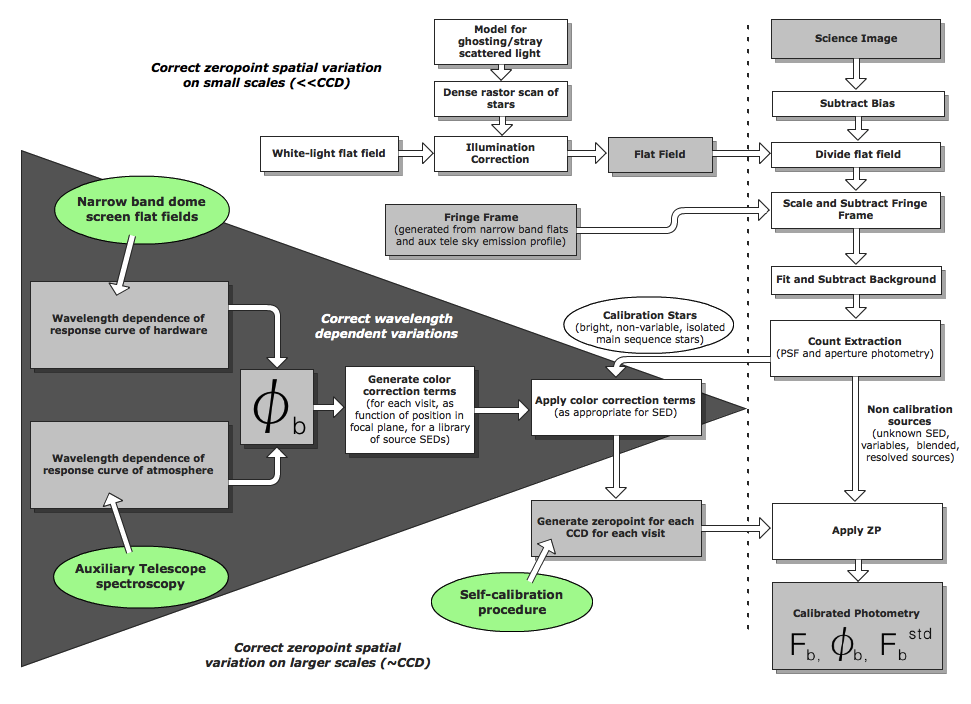
\includegraphics[width=6.5in]{calib_overview}
\caption{ {\small {\bf A flowchart of the Data Release photometric
      calibration process.} Everything to the left of the dashed line
    could be thought of as a calibration product, to be applied to
    data from each visit on the right of the dashed line. Each of the
    darker gray boxes indicates data or calibration products required
    to reach the final goal: calibrated photometric measurements. The
    light green circles point out significant LSST-specific calibration
    systems. The separation of the measurement and correction for 
    wavelength dependent (shape) and wavelength independent
    (normalization) variations in the throughput can be seen in the
    three sections of the `calibration products' on the left hand
    side. The upper portion, consisting mainly of flat-field effects,
    corrects primarily for small spatial scale gray-scale variations (although
    the illumination correction can have larger spatial scale
    structure), the middle portion in the dark triangle corrects only
    for bandpass shape variations, while the bottom portion,
    consisting of the zeropoint corrections calculated from the
    self-calibration procedure, will only correct for larger spatial
    scale variations. }
\label{fig:overview_flowchart} }
\end{figure}

The rest of this section will provide a more in-depth overview of the
calibration measurements required. We will start with a review of what
is physically happening to photons in their path toward the focal
plane (the `truth'), and then outline how LSST will translate the
measured ADU counts back to photons above the atmosphere (the
calibration `model').

\subsection{Truth: From photons to counts}

Let us first consider how the photons from an astronomical object are
converted into ADUs in the detector, paying attention to the various
temporal or spatial scales for variability might arise in the LSST
system to affect the final ADU counts (and ignoring errors in
measurement, as this is the `truth' of the flux transmission). This section is intended
to motivate the separate measurement of the normalization and shape of
the bandpass and introduce some important concepts, such as the
normalized system response.

Given $F_\nu(\lambda, t)$\footnote{Hereafter, the units for specific
flux are Jansky (1 Jy = 10$^{-23}$ erg cm$^{-2}$ s$^{-1}$
Hz$^{-1}$). The choice of $F_\nu$ vs. $F_\lambda$ makes the flux
conversion to the AB magnitude scale more transparent, and the choice
of $\lambda$ as the running variable is more convenient than the
choice of $\nu$. Note also, while $F_\nu(\lambda,t)$ (and other
quantities that are functions of time) could vary more quickly than
the standard LSST exposure time of 15s, it is assumed that all such
quantities are averaged over that short exposure time, so that $t$
refers to quantities that can vary from exposure to exposure. }
the specific flux of an astronomical object at
the top of the atmosphere, at a position described by ($alt$,$az$),
the total flux from the object transmitted through the atmosphere to the telescope pupil is
\begin{equation}
\label{eqn:Fpupil}
   F_\nu^{pupil}(\lambda,alt,az,t) = F_\nu(\lambda, t) \, S^{atm}(\lambda,alt,az,t),
\end{equation}
where $S^{atm}(\lambda,alt,az)$ is the (dimensionless) probability that a photon of 
wavelength $\lambda$ makes it through the atmosphere,
\begin{equation}
\label{eqn:atmTau}
   S^{atm}(\lambda,alt,az,t)   = {\rm e}^{-\tau^{atm}(\lambda,alt,az,t)}.
\end{equation}
Here $\tau^{atm}(\lambda,alt,az)$ is the optical depth of the
atmospheric layer at wavelength $\lambda$ towards the position
($alt$,$az$). Observational data \citep{Stubbs2007b, Burke2010b} show
that the various atmospheric components which contribute to absorption
(water vapor, aerosol scattering, Rayleigh scattering and molecular
absorption) can lead to variations in $S^{atm}(\lambda,t)$ on the
order of 10\% per hour. Clouds represent an additional gray (non-wavelength
dependent) contribution to $\tau^{atm}$ that can vary even more
rapidly, on the order of 2--10\% of the total extinction at $1^{\circ}$
scales within minutes \citep{Ivezic2007}.

Given the above $F_\nu^{pupil}(\lambda,alt,az,t)$, the total ADU
counts transmitted from the object to a footprint within the field of
view at ($x$, $y$) can be written as
\begin{equation}
\label{eqn:Fpupil2counts}
    C_b(alt, az, x,y,t) = C \, \int_0^\infty {F_\nu^{pupil}(\lambda,alt,az,t) \, S_b^{sys}(\lambda,x,y,t) \lambda^{-1}d\lambda}.
\end{equation}
Here, $S_b^{sys}(\lambda,x,y,t)$ is the (dimensionless) probability
that a photon will pass through the telescope's optical path to be
converted into an ADU count, and 
includes the mirror reflectivity, lens transmission, filter
transmision, and detector sensitivity. The term
$\lambda^{-1}$ comes from the conversion of energy per unit frequency
into the number of photons per unit wavelength and $b$ refers to a particular filter, $ugrizy$. The
dimensional conversion constant $C$ is
\begin{equation}
\label{eqn:Cconstant}
        C = {\pi D^2 \Delta t \over 4 g h }  
\end{equation}
where $D$ is the effective primary mirror diameter, $\Delta t$ is the
exposure time, $g$ is the gain of the readout electronics (number of
photoelectrons per ADU count, a number greater than one), and $h$ is
the Planck constant. The wavelength-dependent variations in
$S_b^{sys}$ generally change quite slowly in time; over periods of
months, the mirror reflectance and filter transmission will degrade as
their coatings age. A more rapidly time-varying wavelength-dependent
change in detector sensitivity (particularly at very red wavelengths
in the $y$ band) results from temperature changes in the detector, but
only on scales equivalent to a CCD or larger.  There will also be
wavelength-dependent spatial variations in $S_b^{sys}$ due to
irregularities in the filter material; these are expected to vary
slowly from the center of the field of view to the outer edges,
equivalent to a bandpass shift on the order of 1-2\% of the effective
wavelength of the filter. Wavelength-independent (gray-scale)
variations in $S_b^{sys}$ can occur more rapidly, on timescales of a
day for variations caused by dust particles on the filter or dewar
window, and on spatial scales ranging from the amplifier level,
arising from gain changes between amplifiers, down to the pixel level,
in the case of pixel-to-pixel detector sensitivity variations.

From equation~\ref{eqn:Fpupil2counts} and the paragraphs above, we can
see that the generation of counts $C_b(alt,az,x,y,t)$ from photons is
imprinted with many different effects, each with different variability
scales over time, space, and wavelength. In particular the
wavelength-dependent variability (bandpass shape) is
typically much slower in time and space than the gray-scale variations
(bandpass normalization). These different scales of variability
motivate us to separate the measurement of the normalization of
$S_b^{sys}$ and $S^{atm}$ from the measurement of the
wavelength-dependent shape of the bandpass.

\subsubsection{Normalized bandpass response, $\phi_b(\lambda)$}
\label{sec:phi}

This then leads us to introduce a `normalized bandpass response
function', $\phi_b^{obs}(\lambda,t)$, that represents the true
bandpass response shape for each observation,
\begin{equation}
\label{eqn:PhiDef}
   \phi_b^{obs}(\lambda,t) =  {
     {S^{atm}(\lambda,alt,az,t)\, S_b^{sys}(\lambda,x,y,t) \,
       \lambda^{-1}} \over
     \int_0^\infty { {S^{atm}(\lambda,alt,az,t) \,
         S_b^{sys}(\lambda,x,y,t) \, \lambda^{-1}} \,d\lambda}}.
\end{equation}
Note that $\phi_b$ only represents {\it shape} information about the
bandpass, as by definition
\begin{equation}
\int_0^\infty {\phi_b(\lambda)  d\lambda}=1. 
\end{equation}
Using $\phi_b^{obs}(\lambda, t)$ we can represent the (true, total)
in-band flux of an object for each observation as
\begin{equation}
\label{eqn:Fb}
F_b^{obs}(t) = \int_0^\infty {F_\nu(\lambda,t) \,\phi_b^{obs}(\lambda,t) \, d\lambda},
\end{equation}
where the normalization of $F_b(t)$ corresponds to the top of the
atmosphere. Unless $F_\nu(\lambda,t)$ is a flat ($F_\nu(\lambda)=$
constant) SED, $F_b^{obs}$ will vary with changes in
$\phi_b^{obs}(\lambda,t)$ due simply to changes in the bandpass shape,
such as changes with position in the focal plane or differing
atmospheric absorption characteristics, {\it even if the source is
non-variable}.

To provide a reported $F_b^{std}(t)$ which is constant for
non-variable sources, we also introduce the `standardized bandpass response
function', $\phi_b^{std}(\lambda)$, a curve that will be defined before
the start of LSST operations (most likely during
commissioning). $\phi_b^{std}(\lambda)$ represents a typical hardware
and atmospheric transmission curve, minimizing the difference between
$\phi_b^{obs}(\lambda,t)$ and the standardized reported bandpass.
Now, 
\begin{equation}
F_b^{std}(t) = \int_0^{\infty} {F_\nu(\lambda,t) \,
  \phi_b^{std}(\lambda) \, d\lambda}, 
\end{equation}
is a constant value for non-variable sources. 

Magnitudes provide an easy way to conceptualize the relationship
between $F_b^{obs}$ and $F_b^{std}$, provided that we define a
`natural magnitude' 
\begin{equation}
\label{eqn:natmag}
m_b^{nat}  = -2.5\, log_{10} \, {F_b^{obs} \over F_{AB}} 
\end{equation}
where $F_{AB}$ = 3631 Jy. The natural magnitude, like $F_b^{obs}$ will
vary from observation to observation as $\phi_b^{obs}(\lambda,t)$
changes, even if the source itself is non-variable. The natural
magnitude can be translated to a `standard magnitude', $m_b^{std}$, as
follows:
\begin{eqnarray}
m_b^{nat} & = &-2.5\, log_{10} \, {F_b^{obs} \over F_{AB}}  \\
& = & -2.5 \, log_{10} \, { \int_0^\infty {F_\nu(\lambda,t) \,
    \phi_b^{obs}(\lambda,t) \, d\lambda} \over F_{AB} }  \\
& = & -2.5 \, log_{10} \, \left( { \int_0^\infty {F_\nu(\lambda,t) \,
    \phi_b^{obs}(\lambda,t) \, d\lambda} \over \int_0^\infty {F_\nu(\lambda,t) \,
    \phi_b^{std}(\lambda,t) \, d\lambda}} \right) \, \left( {\int_0^\infty {F_\nu(\lambda,t) \,
    \phi_b^{std}(\lambda,t) \, d\lambda} \over F_{AB}} \right) \\
m_b^{nat} & = & \Delta m_b^{obs} + m_b^{std} 
\end{eqnarray}
where $\Delta m_b^{obs}$ varies with the {\it shape} of the source
spectrum, $f_\nu(\lambda,t)$ and the {\it shape} of the bandpass
$\phi_b^{obs}(\lambda,t)$ in each observation. Note that $\Delta
m_b^{obs}=0$ for flat (constant) SEDs, as the integral of
$\phi_b(\lambda)$ is always one.  For non-variable sources,
$m_b^{std}$ will be non-variable as it represents the throughput in a
standardized bandpass, $\phi_b^{std}(\lambda)$.

The natural and standard magnitudes can be tied back to the counts
produced by the system by adding the correct zeropoint offsets. As
$\Delta m_b^{obs}$ removes all wavelength dependent variations in $m_b^{std}$,
\begin{equation}
\label{eqn:mag2counts}
m_b^{std} = -2.5\,log_{10}(C_b^{obs}) \, + \Delta m_b^{obs} + Z_b^{obs}
\end{equation}
the zeropoint correction here, $Z_b^{obs}$, contains only gray-scale
{\it normalization} effects, such as variations due to the flat field
or cloud extinction. 

Examples of the $\Delta m_b^{obs}$ due to variations in the shape of
the hardware and atmospheric response curves are shown in
Figure~\ref{fig:delta_mags} and Table~\ref{tab:delta_mags}. Two main
sequence stellar models \citep{Kurucz1993} -- one with temperature 35000K
(blue) and one 6000K (red) -- were combined with three different
atmospheric response curves (with X=1.0 with minimal \water vapor,
X=1.2 with a nominal amount of \water (the `standard'), and X=1.8 with
a large \water vapor content) and two different hardware response
curves (one `standard' and one shifted in wavelength by 1\%)
to illustrate the resulting changes in observed natural magnitudes. In
Figure~\ref{fig:delta_mags2}, the $X=1.8$ atmospheric response is
combined with the $1\%$ shift in filter bandpass (altering the
hardware response) for many main sequence kurucz models, spanning a
range of $g-i$ colors, and the resulting changes in natural
magnitudes are plotted.  These examples demonstrate that the scatter in
natural magnitudes induced by expected atmospheric and hardware transmission
curve shape changes alone (without any gray-scale changes) can be larger
than the SRD repeatability requirements would permit. Adding variations 
in the gray-scale normalization due to the hardware response (typically on the
order of 0.01 magnitudes) and cloud extinction (could be up to a few magnitudes)
will increase the scatter in the observed magnitudes. 

\begin{figure}[htbp]
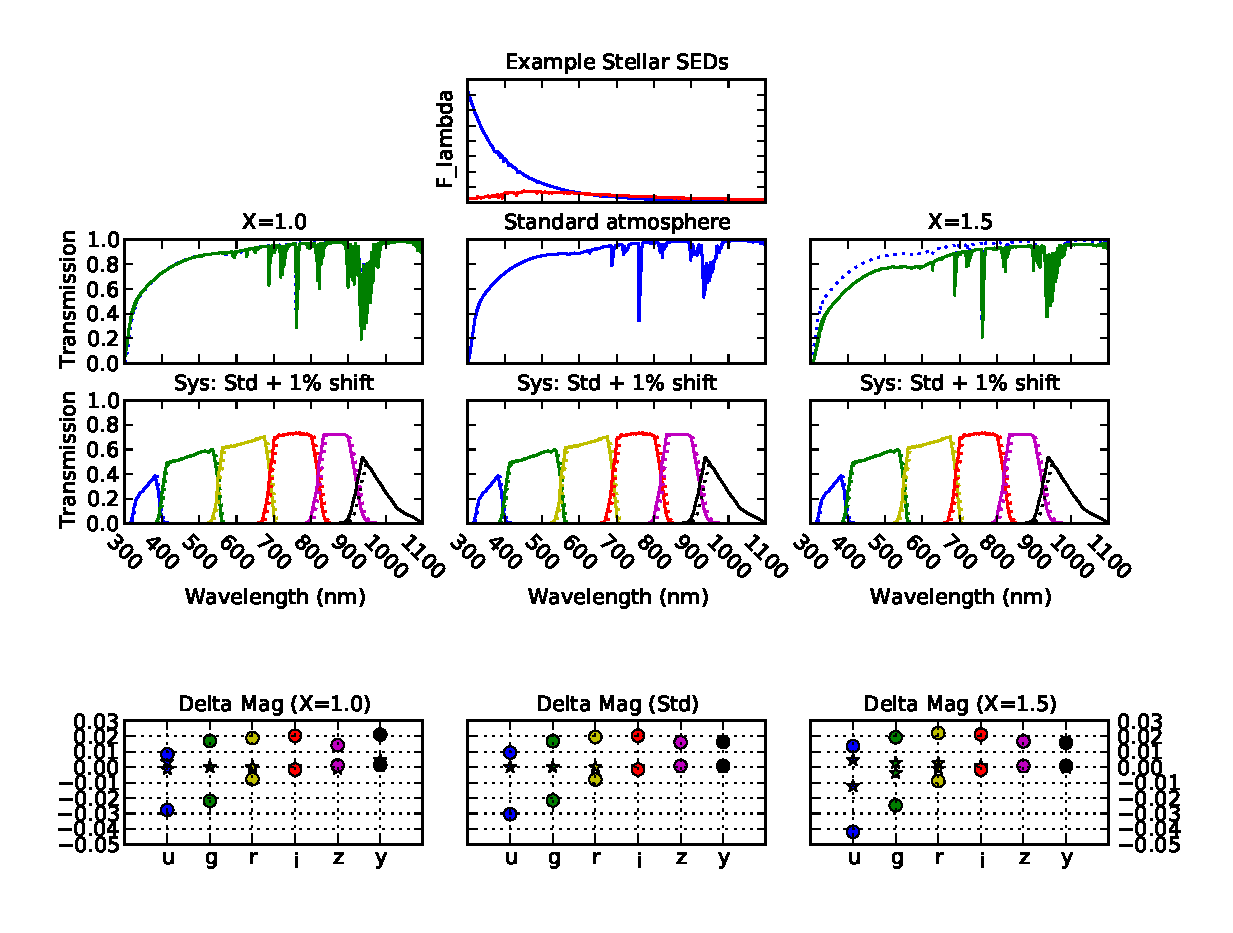
\includegraphics[width=6in]{delta_mags}
\caption{ {\small {\bf $\Delta m_b^{obs}$ due to variations in
hardware and atmospheric bandpass shape.} Two main sequence kurucz model
stars, one blue (35000 K) and one red (6000 K), were used to generate
natural magnitudes (see 
Eqn~\ref{eqn:natmag}) using three different atmospheric transmission
profiles and two different hardware transmission profiles. The stellar
flux profiles are shown in the top center panel, while the atmospheric
transmission functions ($S^{atm}(\lambda)$) are shown across the
second row and the two hardware transmission profiles
($S_b^{sys}(\lambda)$) are duplicated across the third row. The
atmospheric transmission profiles correspond to an airmass=1.0, 1.2
and 1.8 (from left to right), with variable atmospheric absorption
components. The X=1.0 atmosphere is very similar but not
identical to the current LSST default X=1.2 atmosphere throughput
curve, which is used as `standard' here. The hardware transmission
profiles consist of a `standard' profile (matching the LSST current
expected values) and version where the filter throughputs have been
shifted by 1\% of the effective wavelength of each filter (consistent
with the shift expected near the edge of each filter). The final row
demonstrates the changes in observed magnitudes produced by the X=1.0,
`standard' and X=1.8 atmospheres (left to right, respectively),
combined with both the `standard' hardware transmission (represented by
the star points) and the +1\% shifted hardware transmission (represented
by the filled circles) for both the red and blue stars. The exact
differences in magnitudes resulting from this calculation are listed in
Table~\ref{tab:delta_mags}. }
\label{fig:delta_mags} }
\end{figure}

\begin{center}
\begin{table}[htb]
\caption{{\bf $\Delta m_b^{obs}$ due to variations in system and atmospheric
 bandpass shape (see also Fig~\ref{fig:delta_mags}). The first two
rows show the baseline (`standard') magnitude of the star. All other rows show the 
{\it change} in magnitude (in mmag) due to the variations listed at left. } }
\begin{tabular}{l l | c c c c c c}
Bandpass & star &  $u$ (mag) & $g$ & $r$ & $i$ & $z$ & $y$ \\ \hline
Standard (X=1.2) atm, std sys  &  red & 21.472 & 20.378 & 20.000 & 19.911 & 19.913 & 19.913 \\
Standard (X=1.2) atm, std sys  &  blue & 19.102 & 19.503 & 20.000 & 20.378 & 20.672 & 20.886 \\ \hline \hline
 & & $\Delta u$ (mmag) & $\Delta g$  & $\Delta r$  & $\Delta i$ & $\Delta z$  & $\Delta y$ \\ \hline
Standard (X=1.2), +1\% sys shift & red  & -31 & -22 & -8 & -2 & 1 & 1 \\
Standard (X=1.2), +1\% sys shift & blue  & 9 & 17 & 20 & 20 & 16 & 16 \\ \hline
X=1.0, std sys & red  & 7 & 2 & 0 & 0 & -0 & -1 \\
X=1.0, std sys & blue  & -3 & -1 & -1 & -0 & 1 & -4 \\ \hline
X=1.0, +1\% sys shift & red & -24 & -20 & -8 & -1 & 1 & 0 \\
X=1.0, +1\% sys shift & blue & 7 & 16 & 19 & 20 & 18 & 12 \\ \hline
X=1.8, std sys  & red & -21 & -10 & -2 & -0 & 0 & 1 \\
X=1.8, std sys  & blue & 8 & 8 & 4 & 2 & -1 & 6 \\ \hline
X=1.8, +1\% sys shift & red & -50 & -30 & -10 & -2 & 1 & 2 \\
X=1.8, +1\% sys shift & blue & 16 & 24 & 24 & 22 & 15 & 22 \\ \hline
\end{tabular}
\label{tab:delta_mags}
\end{table}
\end{center}

\begin{figure}[htbp]
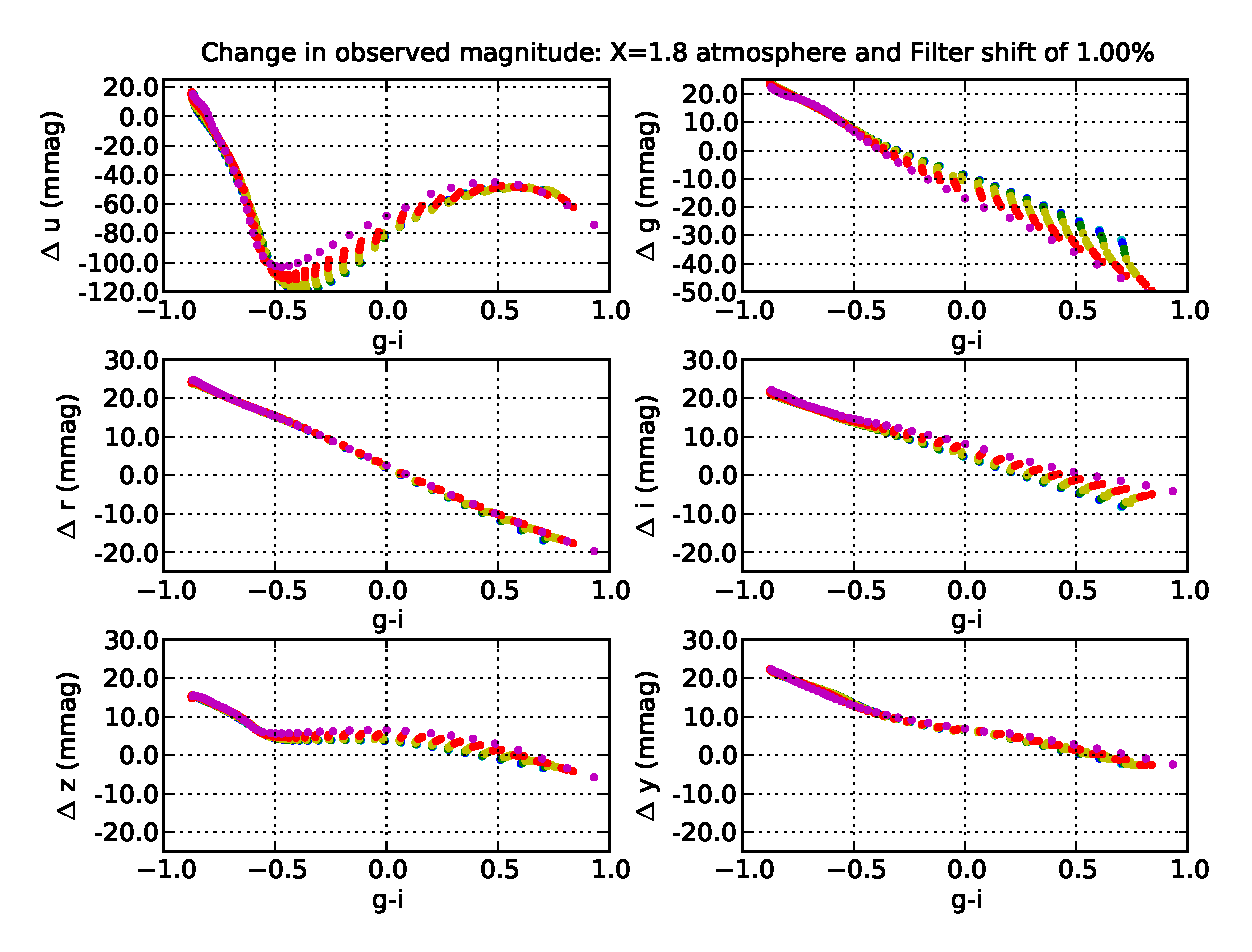
\includegraphics[width=6in]{delta_mags2}
\caption{ {\small {\bf $\Delta m_b^{obs}$ due to
a change in bandpass shape corresponding to a filter shift of $1\%$
and an $X=1.8$ atmosphere.} 850 Kurucz models with temperatures
between 5000K and 35000K and metallicity indexes between -5.0 and 1.0
(solar) were combined with a standard system response (standard
atmosphere and standard hardware bandpasses), then with a total system
response where the atmosphere was replaced by an X=1.8 atmosphere and
the filter component of the hardware transmission was shifted by 1\%
(as in Fig~\ref{fig:delta_mags}). The points in each plot are color-coded by
metallicity, in steps of 1 dex between -5.0 (blue) to 1.0 (magenta).  It can be seen that the
relationship between $\Delta m_b^{obs}$ and $g-i$ can be parameterized,
although generally not with a simple linear relationship. In some
cases (such as seen in the $\Delta u$ and $\Delta g$ panels),
calculating $\Delta m_b^{obs}$ to SRD levels may require more than a simple
$g-i$ color, but this is then primarily a function of metallicity
(which is possible to determine given the $u-g$ color in addition to
the $g-i$ information). }
\label{fig:delta_mags2} }
\end{figure}


\subsection{Model: Calibrating counts}
\label{sec:counts2photons}

The previous section laid out the origins of ADU count variability
from one observation to another. Now we will consider how we can, in
practice, acquire the information necessary to convert a particular
observed ADU count to a measurement of $F_\nu(\lambda,t)$ above the
atmosphere for a particular object.  In other words, how we can
recreate the `truth' by measuring and then compensating for the variations in
$S^{atm}(\lambda,alt,az,t)$ and $S_b^{sys}(\lambda,x,y,t)$, using the
separability of the normalization and shape of the total system
response.

Let us first consider measurement of the variations in the hardware
throughput curve, $S_b^{sys}(\lambda,x,y,t)$. As described in the
previous section, these can be separated into wavelength-independent,
normalization changes which can occur on short (nightly) timescales,
and wavelength-dependent, shape changes which occur over a longer
timescale. Examples of wavelength-independent changes include movement
of dust particles on an optical surface or change in the gain of an
amplifier channel. Examples of wavelength-dependent changes include
the variations in the filter bandpass across the focal plane or
deterioration of coatings on mirrors or lenses over time. We measure
and correct for these variations in different ways.

We can measure the rapidly time variable gray-scale relative
normalization changes in the hardware using standard white-light flat
fields acquired at the start and end of each night through each
filter, in a manner similar to traditional dome flats. This is
discussed in detail in section~\ref{sec:hardware_norm}. 

To measure the wavelength-dependent shape of the hardware response
curve as a function of position in the focal plane, we will use a
dome-screen system that is capable of producing light at a range of
individual wavelengths - producing a data cube of `narrow band flat
fields'.  At each $x$,$y$ location in the focal plane, this data cube
records $\phi_b^{sys}(\lambda,t)$. While this data cube of narrow band
flats could potentially be used as a `synthetic flat field' by
combining the individual narrow band flats according to a chosen
spectral energy distribution, generation of the entire data cube of
narrow band flats is too time-consuming to complete on a daily
basis. Instead, the full narrow band flat field scan will only be
repeated every 30 days, a time interval adequate for measurement of
the more slowly variable $\phi_b^{sys}(\lambda,t)$. This measurement
is discussed in detail in section~\ref{sec:hardware_phi}.

These calibration stages are particularly important for corrections at
very small size scales.  All later calibration stages depend on
photometric measurements of stars, thus can only contribute to
calibration at scales larger than the Point Spread Function (PSF).

It is worth noting that before these flat fields (both the white-light
and the narrow band flats) can be used to measure $S_b^{sys}$, they
must be modified to correctly produce {\it photometrically} uniform
measurements of stars of a defined reference SED across the field of
view. This correction is called the `illumination correction'.  The
illumination correction must correct the observed flat fields for
effects resulting from non-uniform illumination of the dome screen,
for the effect of pixel scale variations across the field of view, for
ghosting caused by internal reflections in the camera, and for the
presence of stray or scattered light arriving in the focal plane on
non-optical paths. See figures~\ref{fig:flatfield} and
\ref{fig:iceffect} for a visual example of the illumination correction
and its importance to image processing. The illumination correction
will be wavelength dependent; for the narrow band flat fields, an
illumination correction for each wavelength must be generated.  The
illumination correction (including ghost corrections) will be
generated by combining measurements of bright, dense star fields
rastered across the field of view during specialized observing
sequences and further corrections generated by the self-calibration
stage (discussed below in section~\ref{sec:hardware_norm}). For the
narrow band flat fields, forward modeling (ZEMAX modeling, constrained
with measurements from the `camera calibration optical bench' (CCOB)
and/or with measurements where the dome screen was illuminated in
narrow band mode at a single location only) will be used to generate
models of the ghost patterns at each wavelength, again with some
further corrections generated by the self-calibration stage (discussed
below in section~\ref{sec:hardware_phi}).  The illumination correction
is expected to be stable with time and will be remeasured only when
the optical path of the telescope is altered. 

Next, considering $S^{atm}(\lambda,alt,az,t)$, we will again separate
the measurement of the shape of the atmospheric response and the
measurement of normalization of the transmission.  The
wavelength-dependent variations in $\phi^{atm}(\lambda,t)$ change
smoothly over spatial scales larger than the field of view and over
several minutes.  By using an auxiliary telescope equipped with a
spectroscope to observe bright stars with known SEDs, we can measure
atmospheric absorption at a variety of positions in the sky every
5--10 minutes throughout the night. These observations are used as
constraints for MODTRAN atmospheric models, generating representations
of the atmospheric throughput in the form of a set of absorption
components as a function of $alt,az,t$. These components can be
interpolated in time and space to generate a wavelength-dependent
atmospheric absorption profile, $\phi_b^{atm}(\lambda,alt,az,t)$, for
each observation. This process is discussed in detail in
section~\ref{sec:atmo_phi}.  

In order to correct for the higher
frequency gray-scale variations in the relative normalization of
$S^{atm}(alt,az,t)$ due to cloud extinction, we must use the
observations of stars in the images themselves, as the cloud
extinction can vary by 0.01 magnitudes on the scale of a CCD
\citep{Ivezic2007} on timescales as fast as a few minutes. This
`self-calibration' procedure could be thought of as creating a massive
calibration `standard' star catalog, where the calibration stars are
all of the non-variable, main-sequence stars in the science images;
the main difference is that the true magnitudes of the calibration
stars have to be bootstrapped from the many different observations of
the survey. For every main sequence star identified as non-variable,
isolated, and in the desired (bright) magnitude range, corrections for
the white-light flat field and $\phi_b^{sys+atm}(\lambda,t)$ must be
applied to produce a standardized magnitude, $m_b^{std}$, then in the
self-calibration procedure we minimize the difference between the
standardized magnitude and a model magnitude,
\begin{equation}
\label{eqn:chi2}
\chi^2 = \Sigma_{ij} \left( { m_{b,ij}^{std} - m_{b,ij}^{model} \over
\sigma_{b,ij}^{std} } \right)^2
\end{equation}
where the model magnitude is derived from the best-fit `true'
magnitude of the calibration star and a model describing how we expect
the magnitude to vary from observation to observation. In the simplest
self-calibration plan, this model simply consists of a normalization constant
(zeropoint offset) for a `patch' equivalent to the size of a CCD,
\begin{equation}
\label{eqn:modelmag}
m_{b,ij}^{model} = m_{b,i}^{best} - \delta z_{b,j}.
\end{equation}
This produces best-fit magnitudes for the calibration star catalog as
well as zeropoint offsets (normalization constants) for each CCD in
every observation, allowing us to correct for atmospheric extinction
on the scale of a CCD. By adopting a more complex model, this
procedure can also correct for variations in the relative
normalization of the total system throughput beyond those contributed
by cloud extinctio (such as remaining errors in the illumination
correction), but is generally limited by the number of stars and
number of observations of each star that are obtained. A CCD size
patch provides about 100 stars per patch, allowing good signal to
noise when determining cloud extinction which varies from observation
to observation, but longer term effects (such as the illumination
correction) may be possible to determine on scales down to approximately
the PSF.  This is similar in nature to the ubercal method applied to
SDSS in \citet{Padmanabhan2008}, and is discussed in more detail in
section~\ref{sec:atmo_norm}.


Repeating Equation~\ref{eqn:mag2counts} above, adjusting ${obs}$ indexes to ${meas}$ to 
reflect the difference between the true and measured quantities,
\begin{equation}
\label{eqn:magsFromCounts}
m_b^{std} = -2.5\,log_{10}(C_b^{meas}) \, + \Delta m_b^{meas} + Z_b^{meas} 
\end{equation}
we can relate the terms in this equation to the corrections just
described above.  $\Delta m_b^{meas}$ originates from the difference
between $\phi_b^{meas}(\lambda,t,x,y)$ and $\phi_b^{std}(\lambda)$
convolved with the source SED, thus depends on the shape of the total
system response as well as the shape of the source SED. $\Delta
m_b^{meas}$ will be calculated by combining a series of model SEDs
with $\phi_b^{meas}(\lambda,t,x,y)$ at various locations in the focal
plane, creating a lookup table of values to apply to measured
magnitudes.  For many sources (but not calibration stars), LSST will
simply assume that the source has a flat SED, at which point the
$\Delta m_b^{meas}$ values become zero, although users may create
their own SED and correction tables based on their knowledge of the
true SED (see Appendix~\ref{sec:photo_better}).  The $Z_b^{meas}$
zeropoint offset comes from any normalization constants generated by the 
self-calibration procedure (in the simple model, just the $\delta z_{b,j}$ in
equation~\ref{eqn:modelmag} above). 

These standard magnitudes are calibrated for variations in the
observed bandpass shape (where applicable) and relative normalization,
thus are directly comparable from one observation to the
next. However, they are not yet tied to an external physical scale or
from one filter band to another, and thus only define an internally
calibrated LSST magnitude in a particular filter.

To fulfill SRD requirements ~\ref{color_req} and ~\ref{abs_req}, these
internally calibrated natural magnitudes must also be tied from one filter
band to another, and then tied to an absolute external physical scale.
For this, a further set of measurements is needed. In all filters, a
set of spectrophotometric standards must be observed, and calibrated using
the steps described above. Then the known SED is combined with
the standard bandpass shape to generate synthetic color
photometry. The synthetic colors are then compared with the
calibrated measured standard magnitudes to calculate $\Delta_{b-r}$,
the corrections needed to tie measurements in each filter together
(referenced to $r$ band).  At this point, only one final measurement
is necessary to tie the entire system to an external physical scale:
an $r$ band LSST natural magnitude measurement of an absolutely
calibrated source on a photometric night. Although in theory these
last two steps could be done with a single externally calibrated
object, on a single photometric night, a larger set of external
reference objects with well known AB magnitudes will be used to reduce
systematic errors. This defines an AB magnitude,
\begin{equation}
\label{eqn:extmags}
m_b^{AB} = m_b^{std}  + \Delta_{b-r} + \Delta_r
\end{equation}
which can be compared to absolute physical flux scales. 

The sequence for photometric calibration is then:
\begin{enumerate}
\item{Acquire a white-light flat in each filter at the start and end
of each observing night. Generate a full, wavelength-dependent
illumination correction for the flats on a many-monthly basis. Apply
the appropriate illumination correction to the white-light flat. Apply
flat field to images directly.}
\item{After remaining image processing (bias correction, fringe
correction, etc) extract ADU counts of sources from images. }
\item{Acquire the data cube of narrow band flat field images,
approximately monthly. Apply wavelength-dependent illumination
correction. Measure $\phi_b^{sys}(\lambda,t,x,y)$. }
\item{Acquire spectra of known stars on a 5--10 minute timeline
throughout each night, fit for atmospheric absorption coefficients and
generate $\phi_b^{atm}(\lambda,t)$ for each science images. }
\item{Combine $\phi_b^{atm}$ and $\phi_b^{sys}$ with a range of model
SEDs to create lookup tables for $\Delta m_b^{meas}$ at various
locations in the focal plane. }
\item{At appropriate intervals (such as at Data Release), run the
self-calibration procedure, applying $\Delta m_b^{meas}$ to stars
chosen for self-calibration procedure and minimizing $\chi^2$ from
equation~\ref{eqn:chi2}.}
\item{Apply appropriate $Z_b^{meas}$ (and potentially $\Delta
m_b^{meas}$ values) to all objects in Data Release catalog, producing
standardized magnitudes.}
\item{Apply measured corrections $\Delta_{b-r}$ and $\Delta_r$,
producing absolutely calibrated magnitudes.}
\end{enumerate}
This results in calibrated $m_b^{AB}$ values in a standardized
bandpass shape, with above-the-atmosphere fluxes.

\section{The internal calibration process}
\label{sec:calib_details}

The next subsections expand on each of the photometric calibration
steps leading to natural magnitude and standard magnitude measurements
described above, including how each correction is measured, calculated
and applied.  The steps described in this section are applied to each
filter independently. The end result of the internal calibration
process is a record of $m_b^{nat}$ and $\phi_b^{sys+atm}(\lambda)$
measured for each object in each observation. In addition, there will
be a reported spectral energy distribution (SED) assumed for each
object ($f_\nu(\lambda)$) and an associated $m_b^{std}$ that is the
natural magnitude corrected for variations in the bandpass shape. In
cases where the assumed SED is flat, $m_b^{std}$ will be equal to
$m_b^{nat}$.
 
\subsection{Normalization of the hardware transmission}
\label{sec:hardware_norm}

Compensation for variations (in $x,y,t$) in the normalization of the
hardware transmission ($S_b^{sys}$) will be done using a white-light
flat field generated using a broad band source illuminating a
specialized dome screen projector. This is the first step in
photometric calibration and is necessary to correct for variations in
the normalization of $S_b^{sys}$ that are smaller than a few times the
PSF (and in the current calibration implementation, smaller than the
scale of a CCD).

The dome screen projector is an array of projectors mounted in the
dome of the LSST enclosure, specially designed to provide very uniform
illumination to the LSST etendue while minimizing any light straying
beyond the etendue. In addition, the dome screen will be able to
project both broadband and tunable narrow band (essentially
monochromatic) light sources, providing both broadband (white-light)
and narrow band flat fielding capabilities.  More details of the
narrow band flat field capabilities are provided in
section~\ref{sec:hardware_phi}. The dome projector system is different from a
traditional dome screen in that the `screen' is a series of light sources,
rather than a screen reflecting a single light source. 

For both white-light and narrow band flat field flat fields, the
projectors are designed to fill the LSST etendue with a uniform
illumination smoothly varying by less than 1\% across the camera field
of view (corresponding to less than 10\% variability across the
projector surface) and less than 0.25\% on scales smaller than
$0.5^{\circ}$ (a little larger than the size of a CCD). The projectors
will also be designed to limit the extent of light emitted outside the
range of angles seen by the camera to reduce stray light in the flat
fields \citep{Gressler2010}. The broadband light source can be tuned
to have any chosen spectral profile; this will be chosen during
commissioning. For simplicity in discussing the next few sections, let
us assume that this is a flat $F_\nu(\lambda)$ profile.

Although the dome screen is engineered to illuminate the LSST etendue
very uniformly on scales approximately the size of a CCD (the
engineering requirement of less than 0.25\% variability translates to
an RMS variation of 0.7~mmag on these scales), the variability across
the full focal plane will exceed LSST SRD requirements. However, even
if the dome screen illumination were perfectly uniform and no stray or
scattered light entered the telescope, the observed flat field still
{\it cannot} be applied directly to science images with the
expectation of achieving photometric uniformity in measurements of
stellar sources. The difference between the desired `photometric' flat
and the observed flat field is the `illumination
correction'. Generating the illumination correction is discussed next. 

%\begin{figure}[htbp]
%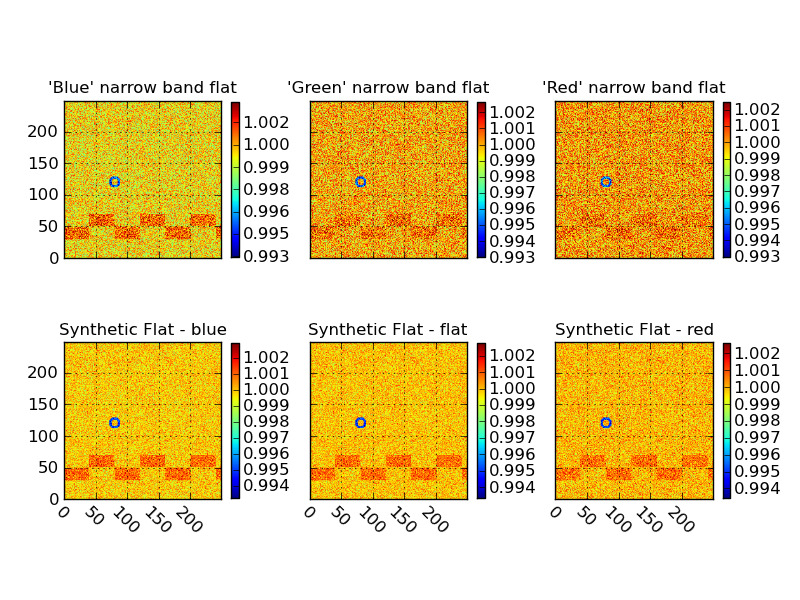
\includegraphics[width=6in]{narrowband_flat}
%\caption{ {\small
%{\bf Simplified examples of synthetic flat generation.} 
%The top panel illustrates simplified narrow band flats, at 'blue',
%'green' and 'red' wavelengths. These represent illumination corrected
%(thus the relatively flat illumination pattern!) narrow band flat
%fields, where the detector shows a sensitivity pattern that is more
%pronounced in the blue wavelength flat field. The bottom panel shows
%the result of combining these flats to create a synthetic flat with a
%desired SED that is either weighted toward blue wavelengths (1.5*blue
%+ 1.0*green + 0.5*red), a completely even distribution, or a synthetic
%flat weighted toward red wavelenghts (0.5*blue + 1.0*green + 1.5*red).
%In operations, the synthetic flat will be created using a well-defined
%SED that will best correct the system normalization for science
%targets in the field. }}
%\label{fig:narrowband}
%\end{figure}


\subsubsection{Generating the illumination correction}
\label{sec:ic}

Generating a truly ideal photometric flat field (for measuring stellar
sources) would require a point source of known illumination at
infinity, extending over an infinitesimally small angular patch of
sky, and movable to any location in the telescope field of view and
observed with no atmosphere -- essentially, a controllable stellar
source. This source's emittance is a Lambertian with uniform surface
brightness that is independent of location on the sky, and it would
emit the same spectral energy distribution (SED) as the source we wish
to measure. We could then raster this point source over the telescope
field of view in steps of a pixel's angular size, and at each location
measure the counts within a fixed aperture centered on the central ray
from those coordinates.  After normalizing the measured array of
intensities to unity, the resulting data can be viewed as an image --
the `ideal photometric flat' for the selected SED.  This would appear
slightly different than a usual flat field image; {\it e.g.} dead
pixels would not stand out, as they would be averaged into each
aperture which overlapped them. When performing photometry, its use
would be slightly different as well; instead of dividing the raw
pixels by the flat, stellar photometry would consist of doing the
aperture sum on the raw pixels and then dividing by the value of the
photometric flat at the aperture center.

In practice, this ideal must be recreated in other ways. Typical
astronomical flat fields generated from dome screens, the twilight sky
or dark sky flats all contain light sources that illuminate the entire
telescope field of view simulateously and is only approximately Lambertian. 
In addition, these sources are only approximately uniform over the field 
of view, and each has an SED which differs from that of the source to be
measured. 

-- WORKING HERE (problem from each of these .. describe ghosting .. describe scattered light,
describe SED problem \& reference bandpass section) - describe how we will generate 
illumination correction using model + `cleanup' with selfcal )
(incorporate some text from below, some from Tim, + new) 



The ideal flat field would demonstrate the hardware response to a
focal plane illuminated exactly as it would be with a dark night sky,
empty of ghosts, glints, stray or scattered light - recreating the
hardware sensitivity variations across the focal plane as well as the
effects of vignetting, both of which must be accounted for in the
science images. The measured flat field, however, not only contains
the actual vignetting and hardware sensitivity variations but also
variations in the actual illumination pattern of the dome screen
projectors, stray light, ghost images of the dome screen, and the
effect of pixel scale variations across the field of view, which must
be removed using the illumination correction. 

The dome screen projectors will be designed to be uniformly
illuminated to 1\% over the focal plane, but this is already beyond
the SRD specifications for photometric uniformity.  There will be also
light scattered within the camera dewar and some fraction of the light
within the etendue will have undergone multiple reflections within the
camera refractive optics (creating `ghost' images of the light from
the dome screen). Estimates by Photon Engineering, Inc. (Tucson, AZ)
indicate that $\approx1-2\%$ of the light that reaches the camera
focal plane may be stray light that did not originate within the LSST
etendue. In addition, projection effects cause a variation in the
pixel scale from the center to the outer edges of the field of view,
so that the pixels subtending a larger area (the center of the field)
gather more light from the dome screen. This effect {\it is} present
in the night sky science images as well, but does not affect the total
flux measured from astronomical objects, so this gradient must be
preserved in the science images (and thus removed from the flat field
through the illumination correction). 

Illlustrative examples of these effects in a theoretical dome flat and
the corresponding illumination correction are shown in
Figure~\ref{fig:flatfield}, and the effect of this illumination
correct on final measured counts are shown in
Figure~\ref{fig:iceffect}.

\begin{figure}[htbp]
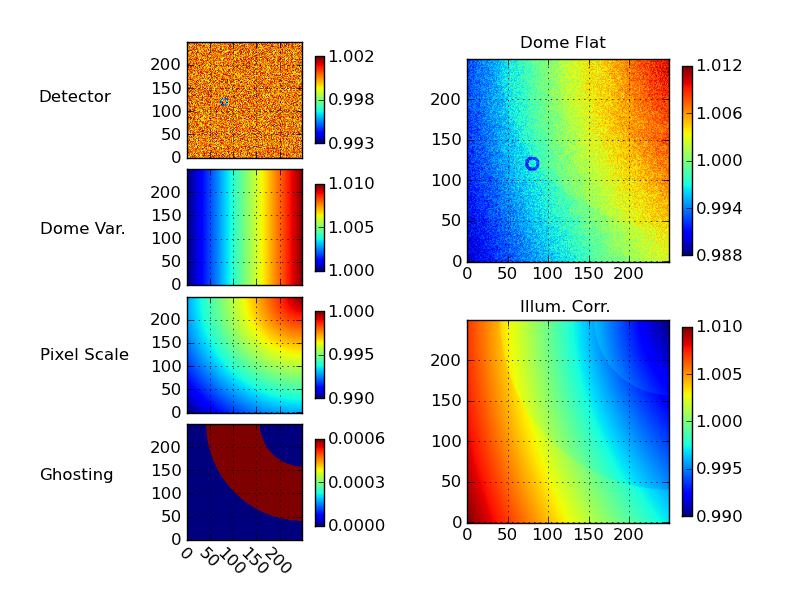
\includegraphics[width=6in]{flatfield_corr}
\caption{ {\small
{\bf Components of the illumination correction.}
Any flat field obtained from the dome screen includes not only a
measurement of small-scale variations in detector sensitivity
(Detector panel, top left), but
also records unwanted effects such as variations in the dome screen
illumination as a function of position (Dome Var. panel), variations in brightness that
result from variations in the amount of sky observed by each pixel
(arising from variations in the pixel scale over the focal plane)
(Pixel Scale panel), and
ghosting caused by internal reflections in the camera (Ghosting panel).
Each panel on the left demonstrates the effect on the total flat field
attributable to each of these variations, in a simplified manner. 
Variations are generated as follows: pixel-to-pixel variation in
detector sensitivity is 0.4\% (as well as a small dust ring), the dome
screen has a 1\% gradient across the field of view, the pixel scale
changes by 0.5\% from corner to corner, and the ghosting is generated
by adding 0.1\% of the total light into a ring reflection. 
The top large panel on the right shows the dome screen flat field that
would be observed after combining all of the effects on the left. The bottom large panel on
the right shows the illumination correction that must be multiplied with 
this flat field to remove the effects of the dome screen variation,
the pixel scale variation, and the ghosting.   Note that no photon noise was
introduced in this simulation. }}  \label{fig:flatfield}
\end{figure}

\begin{figure}[htbp]
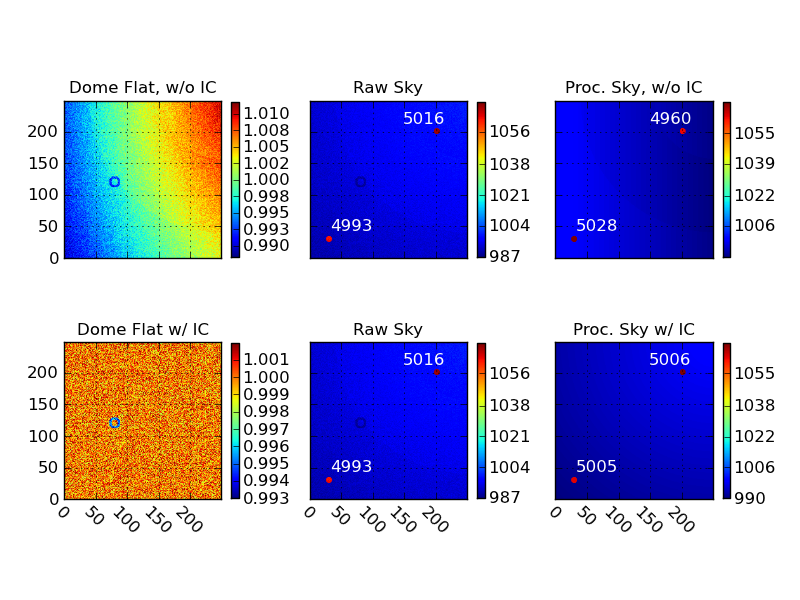
\includegraphics[width=6in]{ICeffect}
\caption{ {\small
{\bf Effect of illumination correction on photometry.}
The left top panel shows a flat field obtained from a dome screen,
creating with the same conditions as in Figure~\ref{fig:flatfield},
without multiplying by an illumination correction. The central top
panel shows a raw `image' of the sky, generated by adding a background
sky value of 1500 counts per pixel (scaled by the pixel area, as in
Fig.~\ref{fig:flatfield}, to two stars. The stars were generated by
placing 5000 counts over a circular aperture the size of the PSF at
the location of the star. A ghost image was created as in
Fig.~\ref{fig:flatfield}.  The right top panel demonstrates the result
of processing the raw sky image by subtracting the ghost image and
then dividing by the dome flat without an
illumination correction. 
The left bottom panel shows the illumination correction applied to the
same flat field. The middle bottom panel shows the same raw sky image as
the top row. The bottom right panel demonstrates an improved processing
of the raw sky image, by subtracting the ghost image and then dividing
by the illumination corrected flat field. 
Note that the sky background does not appear
flat but is correct for preserving stellar photometric accuracy. 
In every image with stars, the numbers next to each star indicate the
counts measured within an appropriate circular aperture for the
star. In the raw images, these counts are not equal because of the
variation in pixel to pixel sensitivities. }} \label{fig:iceffect} 
\end{figure}

Illumination corrections (one per filter) will be generated whenever
the camera is removed from the telescope or the focal path undergoes
significant changes (such as a filter being replaced or the mirrors
being realuminized), but should be stable otherwise. The corrections
will be created by combining information from a ZEMAX model of
ghosting in the camera constrained by measurements from the Camera
Calibration Optical Bench (CCOB), measurements of the observed
individual narrow band dome screen (DS) flats, and dense star fields
rastored across the focal plane on a photometric night.

The first of these components, {\bf Camera Calibration Optical Bench
(CCOB)}, provides a method to calibrate the spatial and
wavelength-dependent response of the focal plane, unmounted from the
telescope, using a well controlled, wavelength-variable, light source
calibrated using a NIST photodiode. This light source, which produces
a spot in the focal plane approximately the size of or smaller than
the PSF, will be scanned across the detector ($x,y$) at a variety of
beam incident angles, ($\theta,\phi$) and at a variety of wavelengths
($\lambda$).  The response of the detector will be measured in two
different configurations: one with only the detector and the dewar
window - which doubles as lens 3 (L3) - and one with the detector, L3,
L2, L1, the filters and the camera shutter. In the L3-only
configuration, the detector response should include only relative
simple ghosting, primarily 3 ghost images from reflections between the
CCD surface and L3. In the full refractive optics configuration (with
L3, L2, L1, the filter and camera shutter), the detector response will
include a more complicated ghost pattern. Current simulations indicate
the strongest ghosts are expected to originate from reflections
between the CCD surface and L3, where the resulting ghosts are
expected to have an amplitude $5\times\approx10^{-4}$ relative to the
flux of the source. Other ghost images, due to reflections between
lens surfaces, should contain about $\approx10^{-5}$ times the flux of
the source.  See Figure~\ref{fig:ghostimage} for an example of
simulated ghosting in the LSST focal plane. These measurements of the
focal plane response in different optical configurations with a known
incoming light source do not directly measure the illumination
correction (for example, neither pixel scale variation due to
projection effects nor the full stray/scattered light from the dome
projectors are included), but it does provide constraints for model
calculations (such as a ZEMAX model) of the illumination pattern in
the camera as a function of wavelength, position in the focal plane,
and beam incident angles, which are necessary for the creation of the
full illumination correction, as well as constrain the focal plane
response itself.

More details about the requirements and physical apparatus of the CCOB
are available in LSST-10015 and LSST-8217.

\begin{figure}
\centering
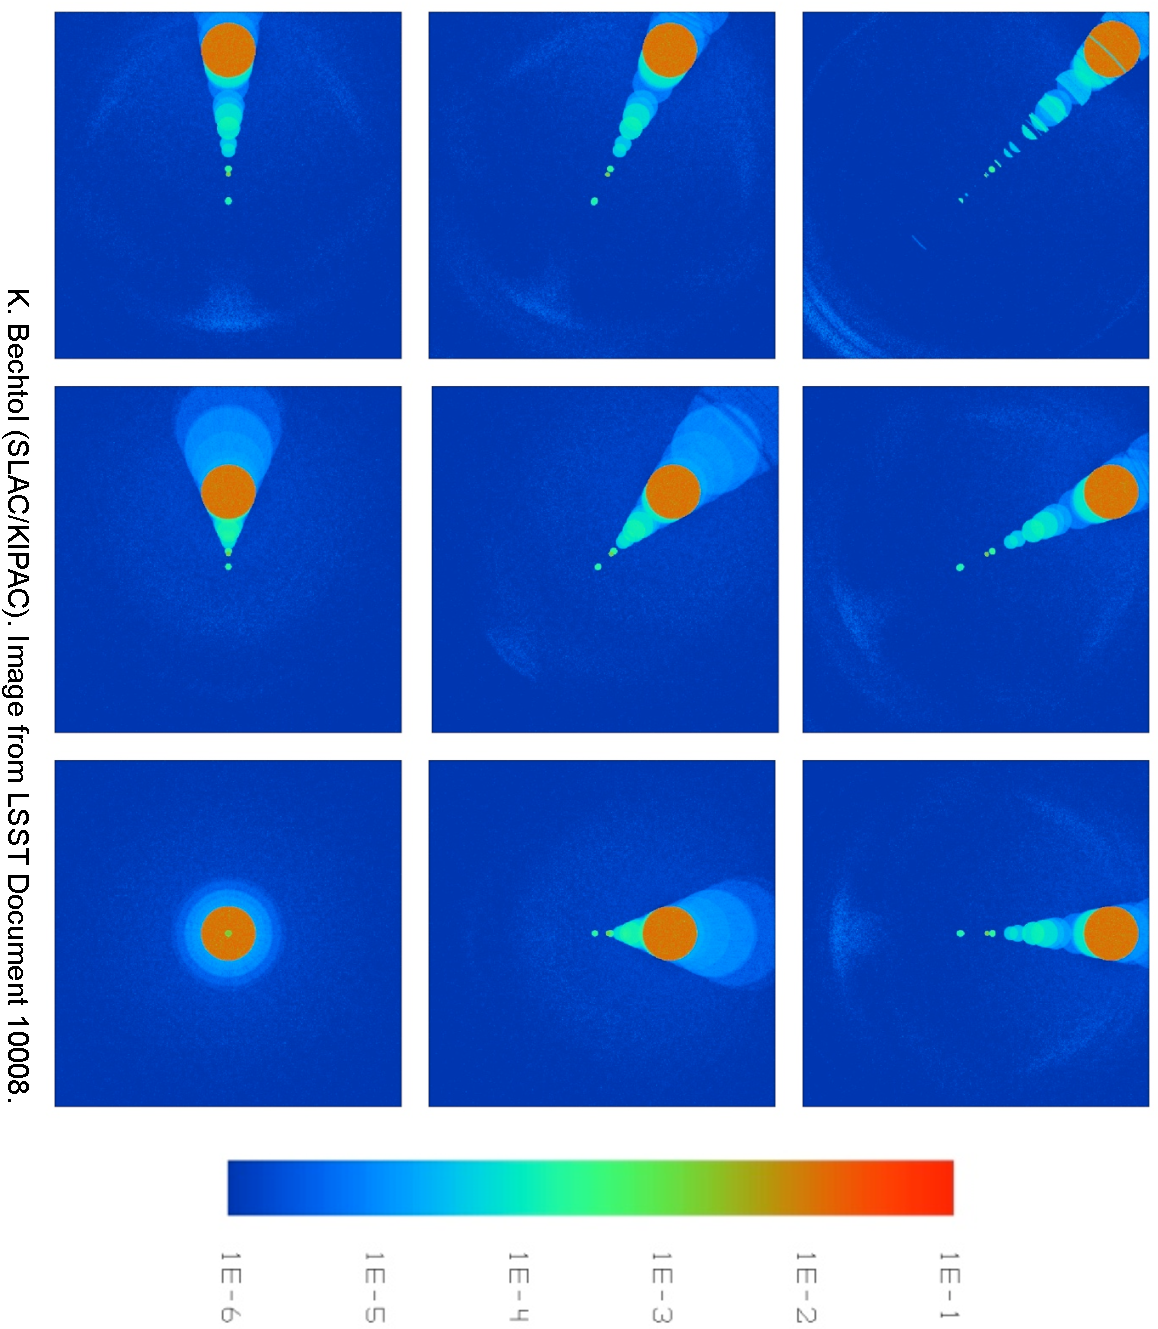
\includegraphics[width=5.5in,angle=90]{ghost_images}
\caption{ {\small
{\bf Simulations of LSST camera ghost images, as measured by CCOB. }
Various beam incident angles, positions and wavelengths will be
explored by the CCOB, creating focal plane measurements similar to
those simulated above. These measurements will be combined to
constrain a ZEMAX model describing the optical paths in the camera
(including the effect of the actual coating reflectivities of the CCD
and lens surfaces, etc). }}
\label{fig:ghostimage}
\end{figure}

The ZEMAX model describes how light scatters inside the camera
creating ghosts at each wavelength. If the dome screen projectors were
perfectly uniform and no stray light was scattered into the LSST
etendue, the narrow band dome flats plus the predictions from the
ZEMAX model would suffice to create a perfect illumination corrected
synthetic flat. Stray light scattered into the LSST etendue can be
modeled using work similar to that of Photon Engineering, Inc., and
then the model constrained by taking measurements of the focal plane
response while blacking out M2 (to image only the stray light). This
creates a preliminary estimate of the illumination correction, which
is particularly useful for small spatial scales (smaller than a CCD)
which may not be well sampled in the next, rastor-scan step.

To account for illumination variations from the dome screen projectors
on large spatial scales (which could be up to 1\% across the field of
view), stray light scattered from other unmodeled surfaces, or systematic
differences in exposure time due to the camera shutter movement,  a dense
network of stars of a variety of spectral types must be rastored
across the focal plane on a photometric night. The images will be
divided by the synthetic flat field corrected by the preliminary
illumination correction, and then the counts for each star corrected
for varying color terms in the atmosphere and hardware response, as
further described in subsection~\ref{sec:phi_correction}.  The final
update to the illumination correction can then be determined by
minimizing over all stars $i$ in all observations $j$,
\begin{equation}
 \chi^2 =  \Sigma_{i=N_{stars},j=N_{obs}} \left( { m_{ij}^{meas}(x,y) - m_{ij}^{model}(x,y)
\over \sigma_b} \right)^2  
\end{equation}
where the model magnitude of each star in each observation is given by
\begin{equation}
m_{ij}^{model}(x,y) =  m_b,i^{best} - \delta k_{b,j}^{atm+sys}(x,y,alt,az,SED,t) - \int d\lambda \, dZ_{IC}(x,y,\lambda)
\end{equation}
where $m_{b,i}^{best}$ is the best-fit, constant magnitude of the star
in this filter, $k_{b,j}^{atm+sys}$ is the color-term correction
(partially determined by the constant from exposure-to-exposure
hardware throughput curve and partially determined by the varying with
each exposure atmospheric throughput curve), and $dZ_{IC}$ is the
update to the illumination correction which is produced by this dense
rastor scan. Similar applications of rastor scans have been
successfully used in previous surveys, ({\it e.g} \citet{Regnault2009,
Magnier2004, Manfroid1996}), providing an illumination correction
accurate to the sub-percent level. With the additional information
from the CCOB and the better intrinsic uniformity of the dome screen
illumination, we expect the illumination correction for LSST to be at
least factor of 2 more accurate.

\subsubsection{Error in the Normalization of the Hardware Transmission}

The dome screen projectors will be designed to be uniform to bertter
than 1\% (10~mmag) across the LSST field of view. After
applying the ZEMAX model to generate expected ghost reflections and
scattering within the camera, and adding dense rastor scans of stars to 
generate a preliminary illumination correction, this variation will be 
reduced to approximately 5~mmag (based on the SNLS experience \citep{Regnault2009}).
With the addition of further improvements from the self-calibration procedure,
we expect the error due to the hardware normalization to be $<3$~mmag. 

%LJ - ok, but actually also .. 10mmag / sqrt(12) to calculate RMS from the *strict* limit, gives
% 3mmag here too ...

\subsection{Correcting for the Shape of the Hardware and Atmospheric
  Response Curve}
\label{sec:phi_correction}

Compensation for the changes in observed magnitudes caused by
variations in the wavelength dependence (shape) of the hardware and
atmospheric response curves, $\phi_b^{sys}(\lambda)$ and
$\phi^{atm}(\lambda)$, will be done using independent measurements of
the hardware response curve (generated from the narrow band flat fields) and the
atmospheric response curve (generated from atmospheric extinction models
generated from measurements from the auxiliary telescope).  While the
measurement of the shapes of the hardware and atmosphere curves are
independent, the actual correction that must be applied depends on the
combination of atmospheric and hardware response curves as well as the
SED of the astronomical object.  This correction is necessary for
precision photometry, but as it requires knowledge of the object's
SED, most LSST reported magnitudes will include either no correction
or a (potentially rough) correction along with an indication of what
SED was assumed to generate this value. However, for stars which will
be used in self-calibration (see subsection~\ref{sec:atmo_norm}) to
determine photometric zeropoints in each exposure, a model SED
well-matched to the object's colors will be chosen and used to
generate the $\Delta m_b^{meas}$ corrections described in this
section.

It is worth emphasizing as we start this section that $\Delta
m_b^{meas}$ is a correction for changes in the {\it shape} of the
bandpass only; any grayscale components to the changes in bandpass
shape discussed here are not part of $\Delta m_b^{meas}$ and instead
belong to either the hardware or atmospheric {\it normalization}
corrections.

\subsubsection{Measuring the shape of the hardware response curve}
\label{sec:hardware_phi}

The dome screen projector system introduced in
section~\ref{sec:hardware_norm} will be used to generate a series of
narrow band flat fields at wavelengths covering the range of LSST's
sensitivity (approximately 350-1100~nm) in each filter.  The same dome
screen uniformity requirements for the white-light flat field apply to
the narrow band dome screen illumination; $<1\%$ across the camera
field of view (corresponding to $<10\%$ variability across the
projector surface) and $<0.25\%$ variability in the focal plane on
scales smaller than $0.5^{\circ}$.

The narrow band light sources can be adjusted at intervals as fine as
1~nm.  A set of precision diodes will be used to normalize the photon
flux integrated during flat field exposures, thus allowing a precise
comparison of the system response at different wavelengths when using
the narrow band light sources.  These photodiodes, together with their
read-out electronics, can be calibrated at the U.S. National Institute
of Standards (NIST) to $\approx0.1\%$ relative accuracy across
wavelengths from 400~nm to 900~nm ($g$, $r$, $i$, $z$ bandpasses)
using current technology.  This can be extended to 1600~nm (into and
beyond the $y$ band) using techniques under development, which also
have the posssibility of achieving 0.01\% accuracy in the diode
calibration at NIST \citep{Eppeldauer09}, as shown in
Figure~\ref{fig:NIST_diode}.

\begin{figure}
\centering
\subfloat[\citet{Stubbs2010a}]{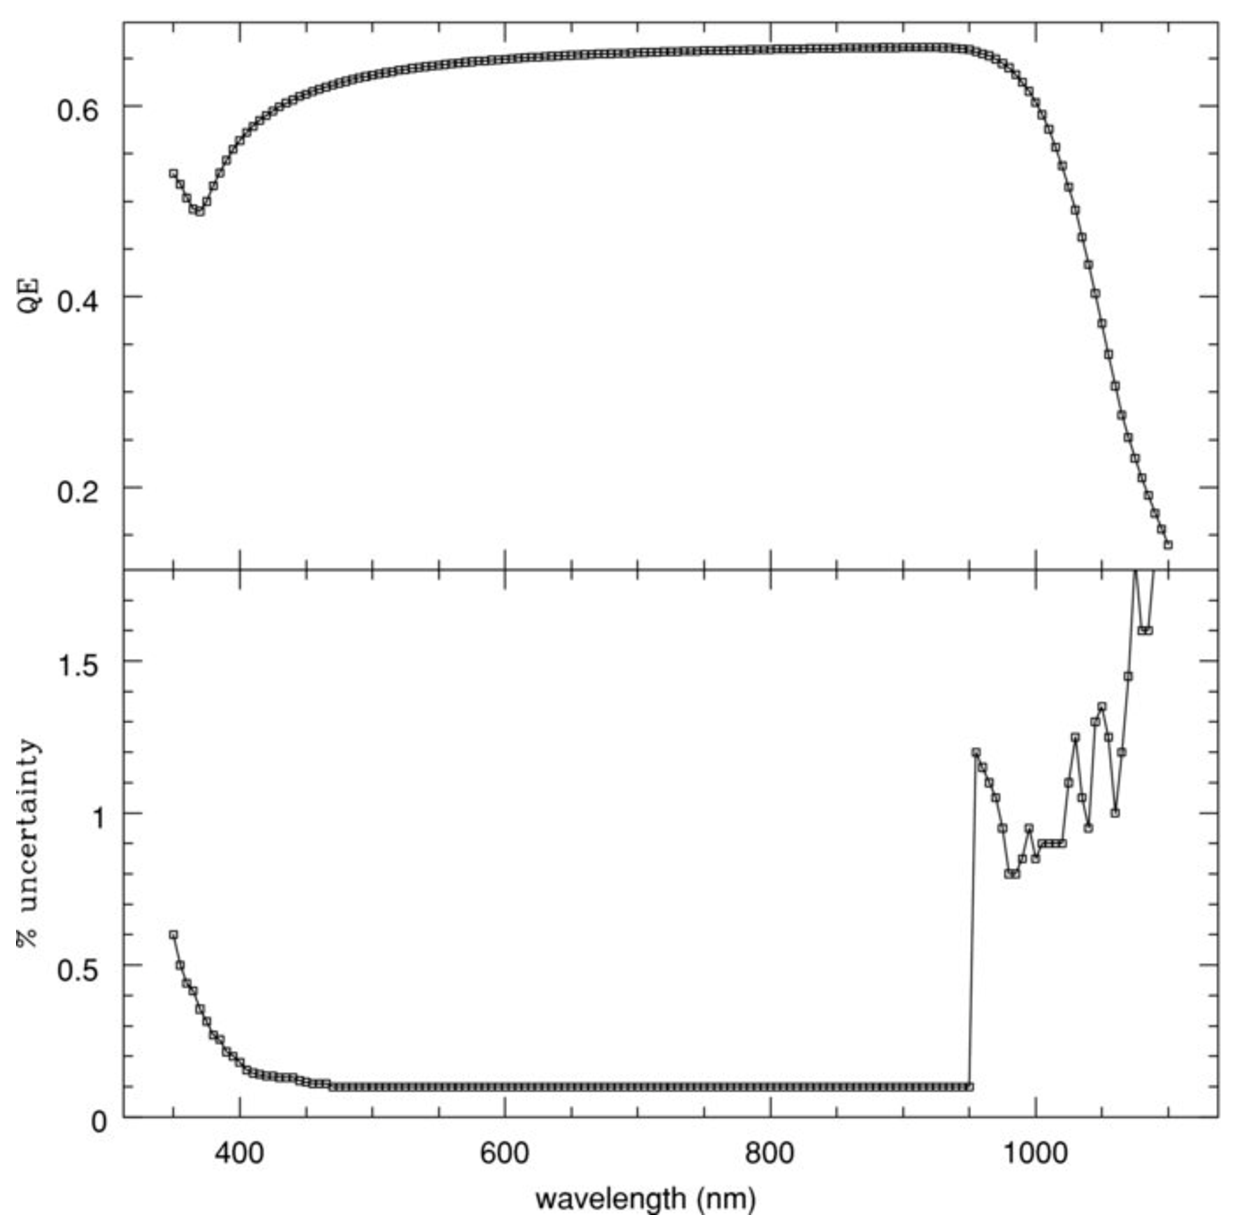
\includegraphics[width=3.5in]{NIST_diode}} \\
\subfloat[\citet{Eppeldauer09}]{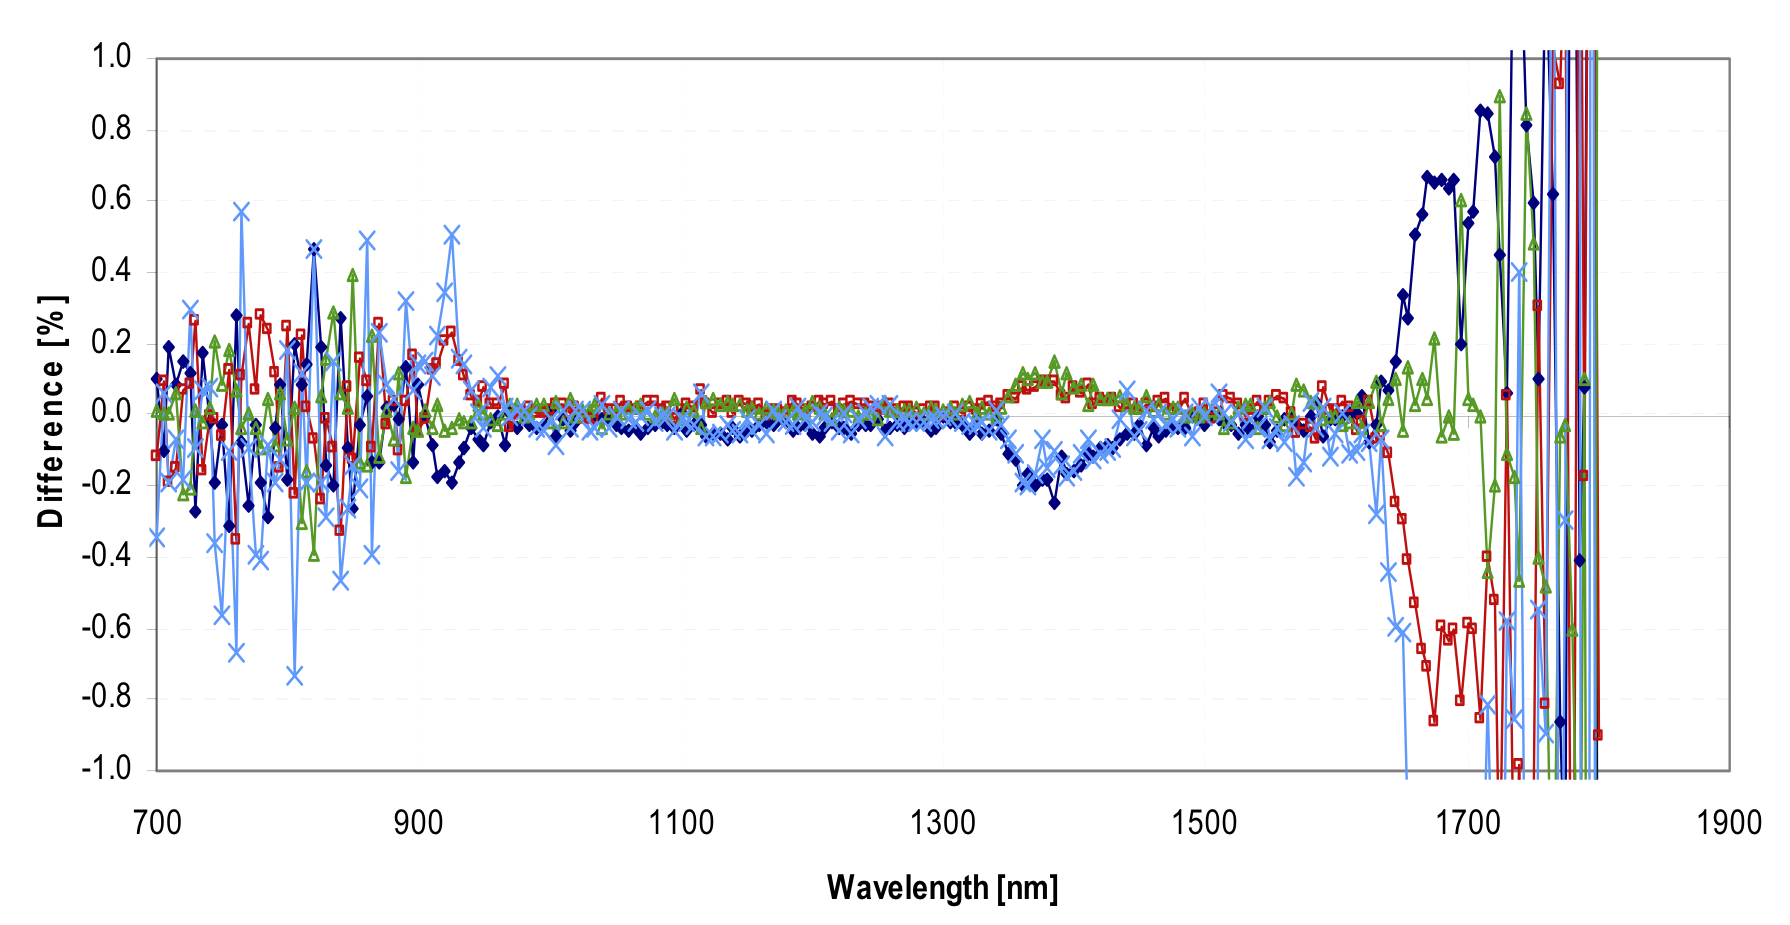
\includegraphics[width=5in]{NIST_diode2}}
\caption{{\small
{\bf Quantum efficiency curve and fractional uncertainty for
NIST-calibrated photodiode, from \citet{Stubbs2010a} and
\citet{Eppeldauer09}.}  Panel (a): Between 400 and 900~nm, calibration
methods already in use in test systems indicate photodiode accuracy is
better than 0.1\%, as in the bottom part of this panel.  The sudden
decrease in calibration accuracy below 900~nm is due to calibration
methods used by NIST in 2005. Panel (b): More recent photodiode
calibration efforts by \citet{Eppeldauer09} show better than 0.1\%
accuracy can be achieved to beyond 1200~nm, the limit of detector
response for LSST, as shown here in the response curves resulting from
multiple scans of a single source using the same photodiode.} }
\label{fig:NIST_diode}
\end{figure}

Further details of the LSST narrow band flat field apparatus can be
found in \citet{Gressler2010}.  Preliminary results from a similar
apparatus tested at PanSTARRS can be found in \citet{Stubbs2010a}, as
well as earlier experiments from CTIO described in
\citet{Stubbs2007a}.

In each filter, a series of narrow band flats will taken at a range of
wavelengths to form a data cube of flat fields in ($x,y,\lambda$). The
narrow band flats are time-consuming to acquire; scanning through all
6 filters at 1~nm intervals requires many hours worth of exposures,
but must also be done in minimal levels of ambient light. Luckily, any
wavelength dependent variations in the synthetic flat are expected to
change relatively slowly so the full set of narrow band flats only
need to be acquired approximately once a month, which could be done
during cloudy nights.

\subsubsubsection{The narrow band flat field illumination correction}

At each wavelength, the narrowband flat field must be illumination
corrected and then used to measure the total hardware response over
all $x,y$ positions, while the photodiodes track the relative intensity of 
the light produced by the dome screen projectors as a function of wavelength.
The illumination correction for the narrow band flat fields suffers from
similar problems as the white-light flat field illumination correction, but
becomes more complicated as ghosting becomes more problematic. 

\subsubsubsection{The expected effect of $\phi_b^{sys}(\lambda)$ variations}

It is expected that the shape
of the response curve will be primarily a function of radius due to
variations in the thickness of the filter coatings caused by the
mechanism used to deposit those coatings. The variation due to filter
nonuniformities is specified to be less than 1\% across the focal
plane, most likely in the form of a bandpass shift as shown in
Figure~\ref{fig:filtershift}. For main sequence stars, the resulting
changes in observed magnitude as the bandpass shifts by 1\% of the
central wavelength can be as much or more than 0.04~magnitudes (40
mmag) - even larger in the $u$ band (see
Figure~\ref{fig:dmag_filtershift}). However, as long as the variation
in the hardware response curve is measured to better than 0.05\% --
equivalent to approximately a 3~Angstrom error in wavelength
calibration of the monochromatic light source throughout the bandpass
or a 0.5\% error in photodiode calibration assuming that the shape of
each bandpass is determined using at least 100 independent
measurements (i.e. 1 measurement every few nanometers within the bandpass) --
the maximum error contribution towards calibrating these observed magnitudes
will be less than 2~mmag for all bandpasses other than $u$, where the
error could be as much as 5~mmag for certain main sequence stars (see
Figure~\ref{fig:dmag_filtershift_small}). 

Because the shape of the hardware response curve varies as a function
of filter radius, it is also necessary to monitor any offsets of the
filter position from dead center after any filter changes. Assuming
the filter response curve varies linearly with radius, the filter
location must be measured to better than 0.025\%  for the filter
positioning to remain less than a 1~mmag source of error. 
%Given the
%filters are approximately 75~cm in diameter, this means the filter 
%positioning must be recorded to better than 0.18~mm. 
%LJ - beamsize 100mm, plus review filter location requirement ... 0.025\% is too small
%Plus need to include shift in bandpass due to change in incident angle ? 

\begin{figure}
\centering
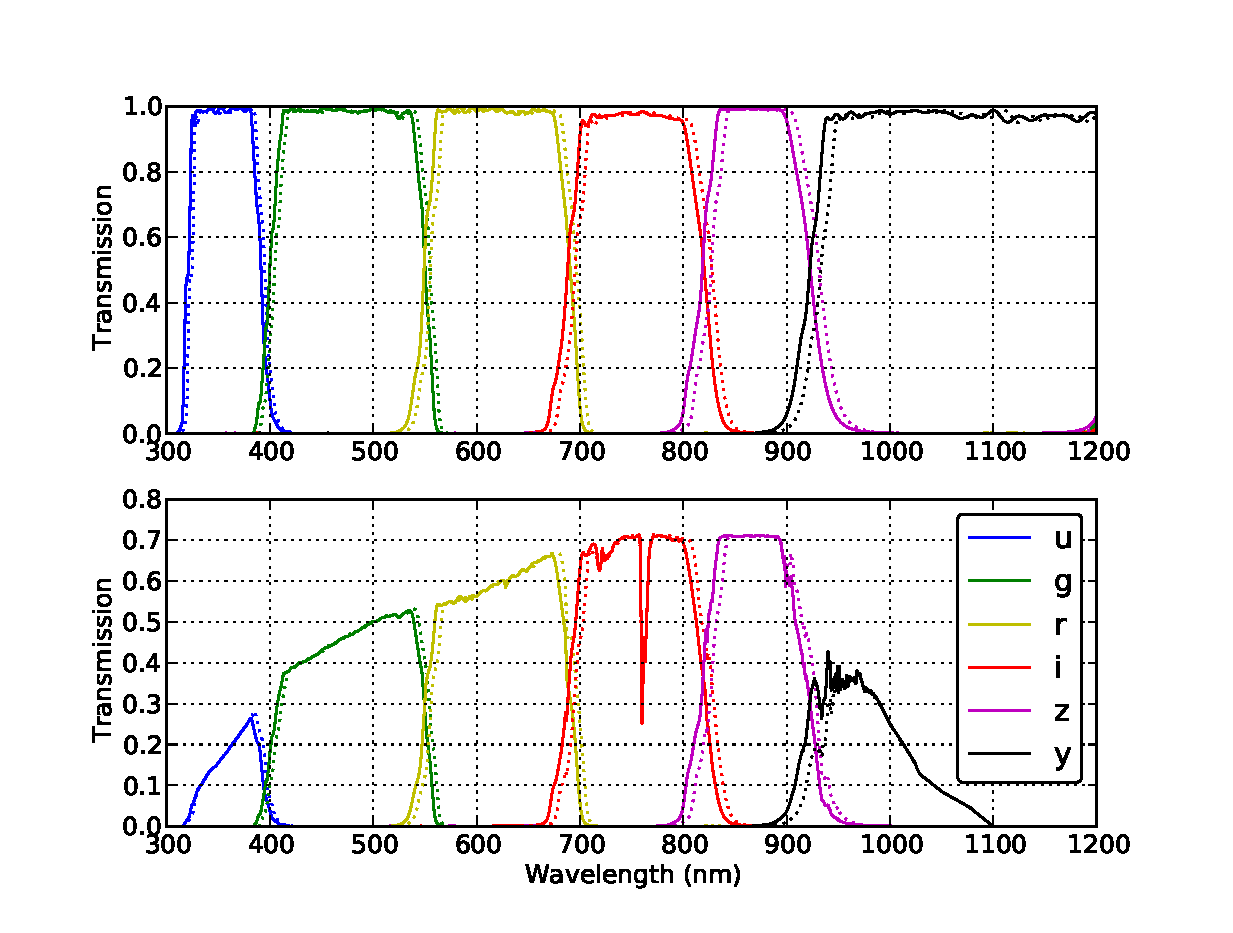
\includegraphics[width=6in]{filter_shifts}
\caption{{\small 
{\bf Baseline filter curves and a potential (1\% of the central
  wavelength) shift due to nonuniformity.}
The solid lines indicate standard filter bandpasses (top panel: filter
alone, bottom panel: filter plus standard mirror, lens, detector and atmosphere
response curves) while the dashed lines indicate the same bandpass
shifted redward by 1\% of the central wavelength.}}
\label{fig:filtershift}
\end{figure}

\begin{figure}
\centering
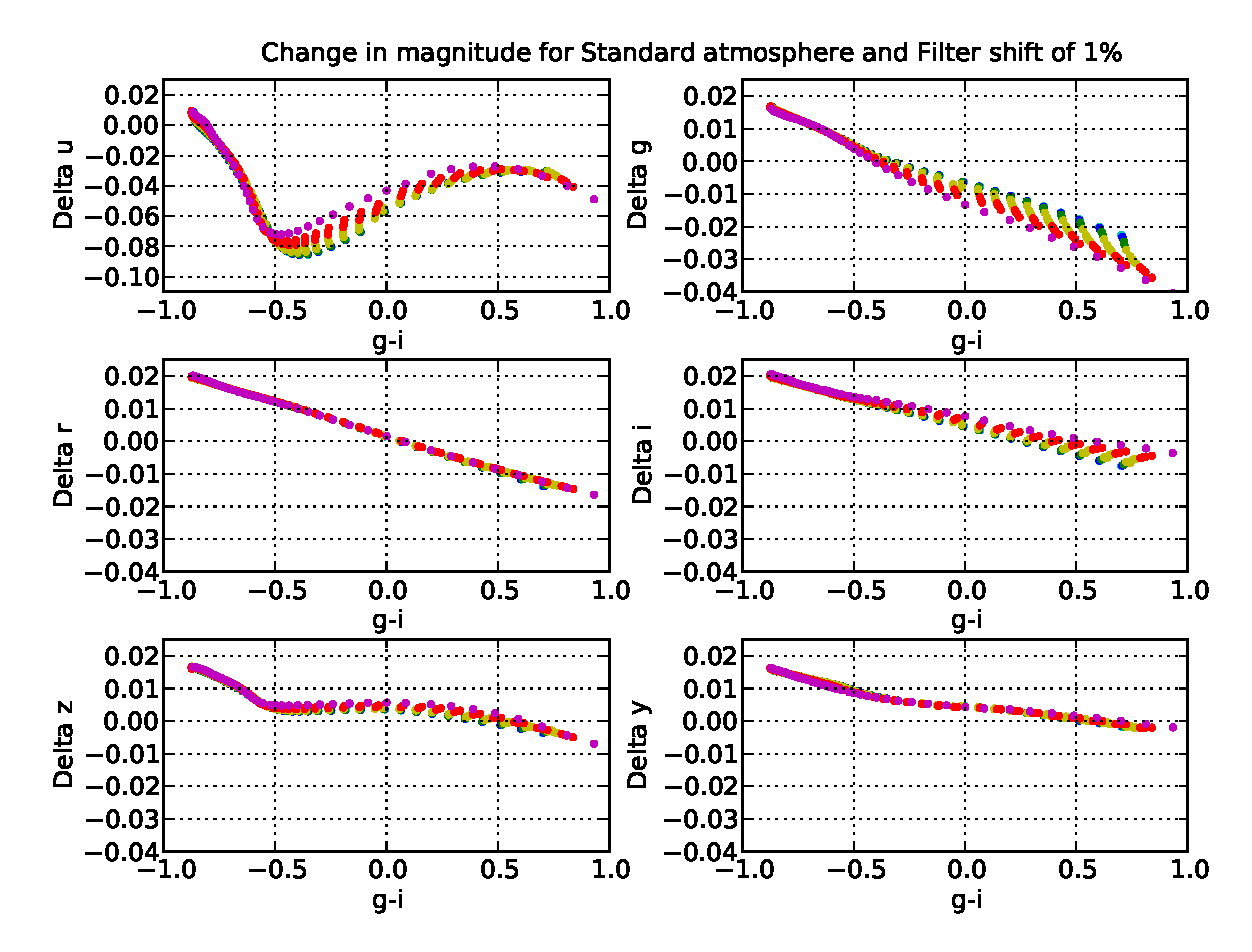
\includegraphics[width=6in]{delta_mags_filtershift}
\caption{{\small 
{\bf $\Delta m_b^{obs}$
due to a hardware response curve shift of 1\% of the central
wavelength of each bandpass.}  850 Kurucz models with temperatures
between 5000K and 35000K and metallicity indexes between -5.0 and 1.0
(solar) were combined with a standard atmosphere and standard
hardware bandpass, and then with a total system response where the
atmosphere remained constant but the hardware response was shifted by
1\% of the central wavelength of each bandpass (as in
Fig~\ref{fig:filtershift}). The points in each plot are color-coded by metallicity, in
steps of 1 dex between -5.0 (blue) to 1.0 (magenta). The resulting
changes in observed 
natural magnitudes are on the order of
20~mmag typically, except in $u$ band where the shift can create a
$\delta u$ of closer to 80~mmag for certain kinds of main sequence
stars. } }
\label{fig:dmag_filtershift}
\end{figure}

\begin{figure}
\centering
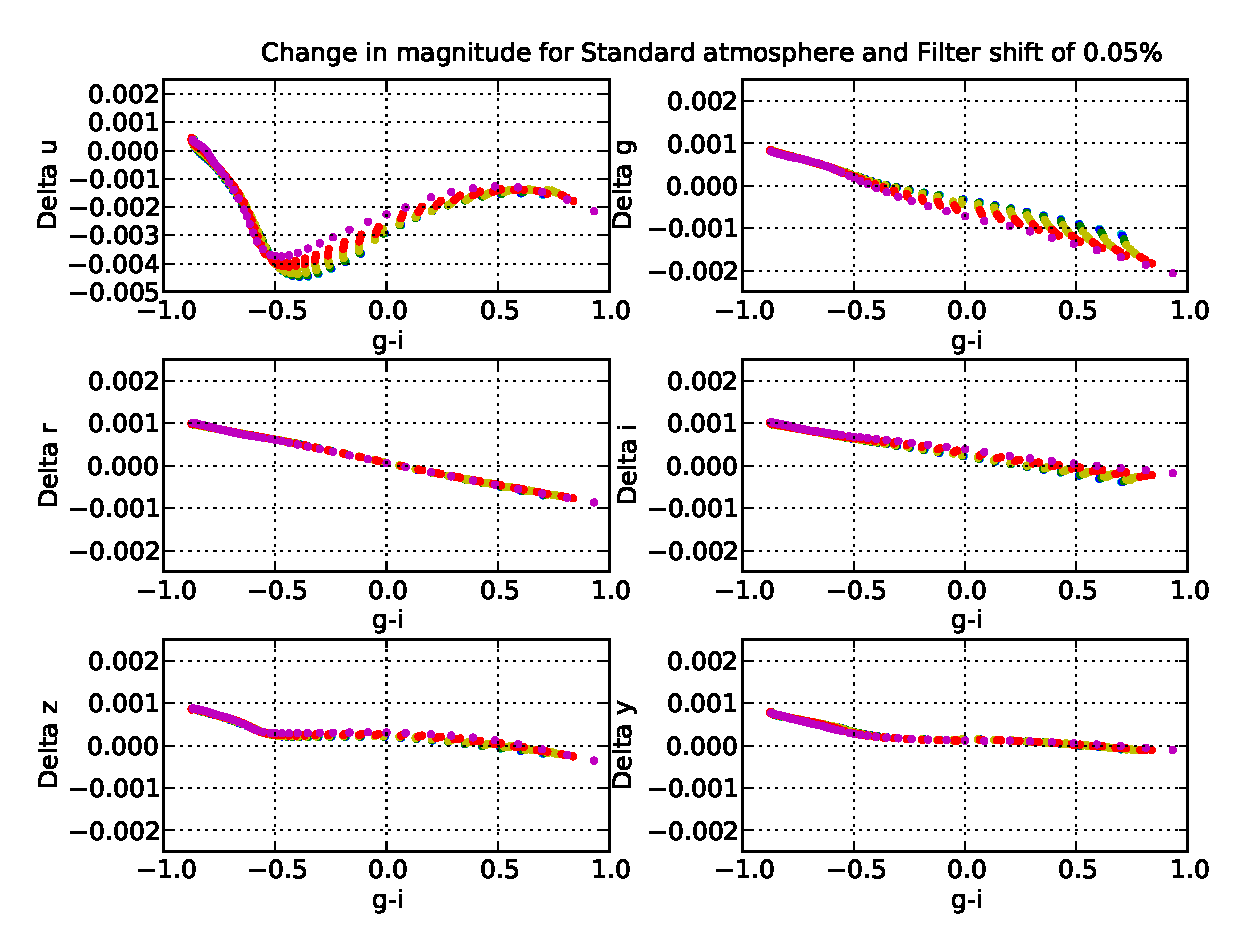
\includegraphics[width=6in]{delta_mags_filtershift_small}
\caption{{\small 
{\bf $\Delta m_b^{obs}$ due to a hardware
response curve shift of 0.05\% of the central wavelength of each
bandpass.} Similar to Fig~\ref{fig:dmag_filtershift} except that the
hardware response was shifted by only 0.05\% of the central
wavelength, an amount representing an unmeasured shift in the hardware
response and thus contributing directly to the final error in the
calibration of the natural magnitudes. Note that the y scale here is 1/10th
of the scale in the previous figure. }}
\label{fig:dmag_filtershift_small} 
\end{figure}
 

\subsubsection{Measuring the shape of the atmospheric transmission curve}
\label{sec:atmo_phi}

The shape of the atmospheric transmission curve appropriate for each observation
will be generated using data from spectroscopic measurements of bright
stars obtained with the LSST auxiliary telescope. These measurements
will be fit to a model of atmospheric absorption extinction (which includes
how this absorption varies across the sky and over time as well as
atmospheric extinction profiles generated by MODTRAN \citep{modtran4a,
  modtran4b}) to determine
the atmospheric transmission profile at all points on the sky at all
times. 

\subsubsubsection{Atmospheric absorption behavior}
\label{sec:atmo_behavior}
The shape of the atmospheric transmission curve, $\phi^{atm}(\lambda,
alt, az, t)$, is determined by three major sources of atmospheric
extinction: molecular scattering (Rayleigh scattering), aerosol
scattering (Mie scattering), and molecular absorption. 
\begin{itemize}
\item{Molecular scattering, or Rayleigh scattering, is due to elastic
scattering off atoms and molecules in the air. Atmospheric absorption
due to Rayleigh scattering has an optical depth 
\begin{equation}
\tau \propto (\lambda/ \lambda_o)^{-4}\, (BP/BP_o),
\end{equation} 
where $BP$ is the barometric pressure \citep{Hansen1974}, and $BP_o$ is a reference value
(typically around 782~mb for Cerro Tololo).  The total atmospheric
extinction due to Rayleigh scattering is thus driven only by pressure
variations and is proportional to airmass, 
\begin{equation}
S(\lambda,X) \propto e^{-\tau, X},
\end{equation} 
and is also axisymmetric around zenith. Changes in the
optical depth due to Rayleigh scattering typically will produce
$<1$~mmag change in the observed counts.}
\item{Aerosol scattering, or Mie scattering, occurs when visible light
is scattered by particles suspended in the atmosphere with a size
similar to its wavelength.  This gives rise to an absorption curve
with a strongly variable total column depth as well as a variable wavelength
dependence, where 
\begin{equation}
\tau \propto (\lambda/675 \rm{nm})^{\alpha}.
\end{equation} 
The index $\alpha$ has been measured to range between -0.9 to -1.7 in
observations from CTIO \citep{Burke2010b}.  From \citep{Stubbs2007b}
optical depth measurements from Mauna Loa, the total aerosol optical
depth at zenith varied from 0 to 0.3 (generally <0.1) at
$\lambda=440$~nm, with max rate of change $\approx0.02$/hr. The
atmospheric extinction due to aerosol scattering scales directly with airmass but is not
necessarily axisymmetric around zenith and often has an East-West
trend.}
\item{Molecular absorption produces a more complex
set of absorption bands and features, originating from line absorption
due to ozone (\ozone), water (\water), oxygen (\oxy) and other trace species
(OH, N$^2$O, etc.). The resulting atmospheric absorption features are largely due
to narrow saturated Lorentzian-shaped lines spaced closely in
wavelength and, due to this saturation, scale non-linearly with
airmass, 
\begin{equation}
S(\lambda, X) \propto e^{-\tau\,\sqrt X}
\end{equation} 
as in \citep{Stubbs2007b}. The total column depth for \oxy and other
trace species is related directly to the square root of the column depth for molecular
scattering, and is thus proportional only to the square root of the
barometric pressure and airmass. However, \ozone and \water absorption
is more variable. \ozone absorption can vary by
5--10\% day to day, with seasonal variations of 25\% or so, but is
expected to be non-variable across the sky and closely correlated with
satellite data on total ozone content. \water absorption can vary on timescales as short as
10--20 minutes, and is expected to show linear trends across the sky
(East-West and North-South). 
}
\end{itemize}
Figure~\ref{fig:absorption_comps} demonstrates the
wavelength dependency of each of these components and how they change
with airmass. 

\begin{figure}[htpb]
\centering
\subfloat[]{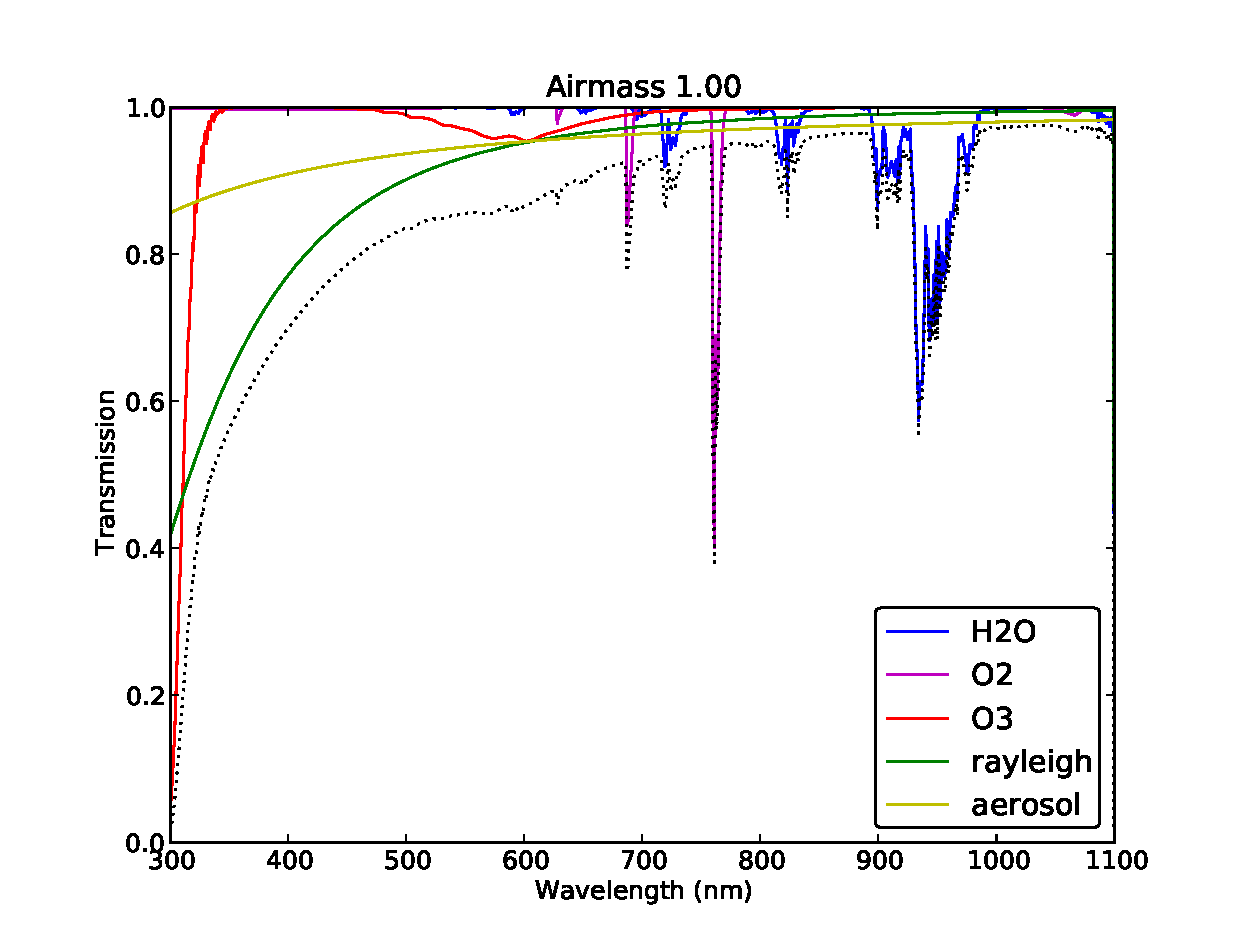
\includegraphics[width=4in]{absorption_compsA}}\\
\vspace{-15pt}
\subfloat[]{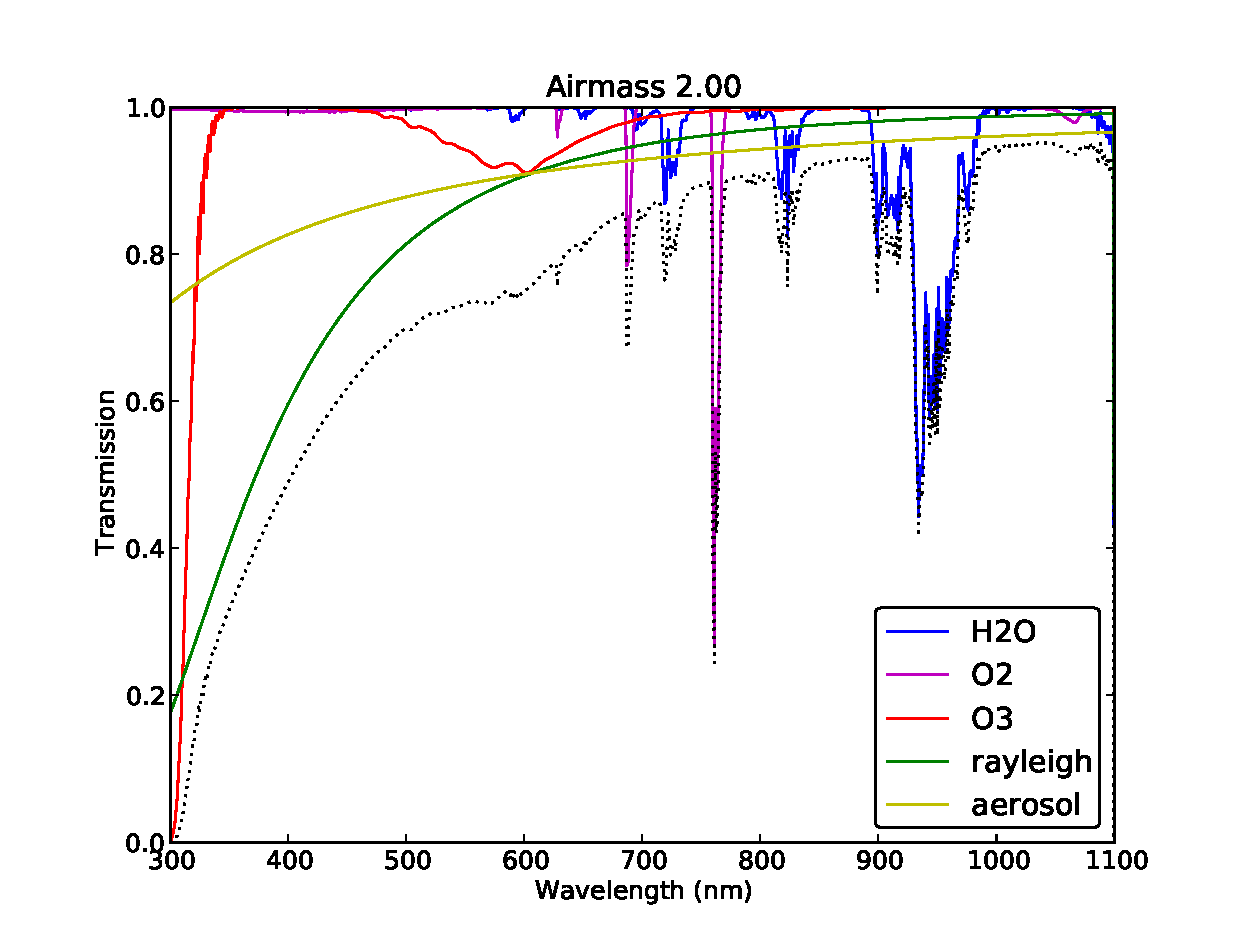
\includegraphics[width=4in]{absorption_compsB}} 
\caption{{\small
{\bf Components of atmospheric absorption.} The wavelength dependence
of the various components of atmospheric absorption at zenith (panel
a) and at airmass=2.0 (panel b) is shown here.  The \water (blue) and \ozone
(red) molecular absorption contributions are shown separately,
while the \oxy absorption is combined with other trace elements (magenta). A
typical example of aerosol scattering (Mie scattering) is included
(yellow), as is molecular scattering (Rayleigh scattering)
(green). All components except aerosol scattering were generated using
MODTRAN4 with the US Standard option (aerosol scattering is not part of the US 
Standard atmosphere). The resulting total absorption curve is the product of each
of these effects and is shown with the dotted black line. This is an
illustrative atmosphere; under actual observing conditions the
molecular absorption components will vary in strength with time and
the square root of the airmass, the molecular and aerosol scattering
will depend on airmass, and the aerosol scattering profile will also 
vary with time.}}
\label{fig:absorption_comps}
\end{figure}

\subsubsubsection{Fitting the atmospheric absorption}
\label{sec:fit_atmo}

\begin{figure}[htb]
\centering
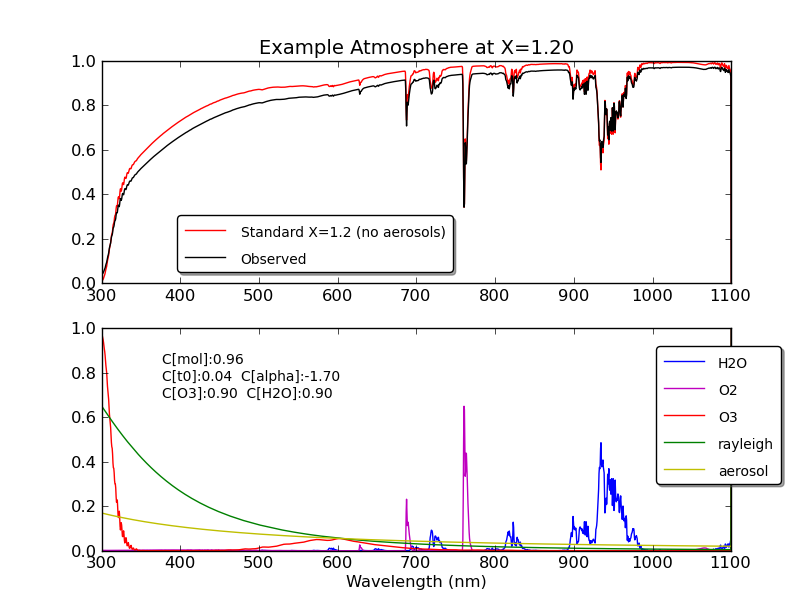
\includegraphics[width=6in]{atmo_airmass12}
\caption{{\small
{\bf Example of an atmosphere generated from a typical mix of
atmospheric components.} The bottom panel shows the MODTRAN absorption
templates at this airmass used in generating the final atmosphere
(the $A_{rayleigh/\oxy/\ozone/\water}$ and $A_{aerosol} = 1-e^{\tau_{aerosol}}$ from
Equation~\ref{eqn:atmo_fit}). The top panel shows the final combined atmospheric
transmission curve in black, as well as a `standardized' atmospheric transmission
curve in red. This demonstrates that (even without using the full
MODTRAN software, just the transmission templates) that we can closely
recreate any atmosphere desired with any composition.} }
\label{fig:absorption_comps2}
\end{figure}

Using MODTRAN we can generate atmospheric transmission profiles at a
variety of airmasses for
each of these major sources of atmospheric extinction -- molecular
(Rayleigh) scattering, aerosol (Mie) scattering, and molecular
absorption from each of \ozone, \water, and combined \oxy/trace species, as is
shown in Figure~\ref{fig:absorption_comps} for a standard atmospheric
composition (the 1976 US Standard). These
profiles capture the wavelength dependence of each component
individually, over a grid of airmasses, and can be used as
templates to generate new atmospheric transmission curves for any
desired atmospheric composition as follows:
\begin{eqnarray}
S^{fit}(alt,az,t, \lambda) & = & \,e^{-\tau_{aerosol}(alt,az,t,\lambda)\,X} \nonumber \\
 & & \times \, (1 - C_{mol}\, (BP(t) / BP_o) \, A_{Rayleigh}(X, \lambda)) \nonumber \\
 & & \times \, (1 - \sqrt{ C_{mol}\, (BP(t) / BP_o)} \, A_{\oxy}(X, \lambda)) \nonumber \\
 & & \times \, (1 - C_{\ozone}(t) \, A_{\ozone}(X, \lambda)) \nonumber \\
 & & \times \, (1 - C_{\water}(alt,az,t)\,A_{\water}(X, \lambda)).
\label{eqn:atmo_fit}
\end{eqnarray}
The $A_{Rayleigh/\oxy/\ozone/\water}$ functions are
absorption templates (i.e. 1 minus the transmission profiles from the
MODTRAN models) and the $C_{mol,\ozone,\water}$ are
coefficients describing the composition of the atmosphere together
with $\tau_{aerosol}$, and $BP(t)$ is measured. An example of an
atmosphere generated in this fashion is shown in
Figure~\ref{fig:absorption_comps2}, demonstrating that this method can
be used to generate an atmosphere at any airmass for any composition
desired, without needing to generate a full MODTRAN model. 

With this capability, we can fit the auxiliary telescope spectroscopic data taken
throughout the night for the values of
$C_{mol,\ozone,\water}$, increasing our SNR for these
coefficients by modeling their expected behavior over time and across
the sky as detailed in \ref{sec:atmo_behavior} above. The Rayleigh
scattering and molecular absorption due to \oxy and other trace
species are fit with a single coefficient, $C_{mol}$, which simply
scales the MODTRAN templates to the appropriate level for Cerro
Pachon, and then only change with the barometric pressure ($BP$). The
\ozone absorption is fit with a single $C_{\ozone}$ value for each
night. The aerosol absorption, as it is expected to have a small
spatial variation across the sky, is modeled as 
\begin{equation}
\label{eqn:tau_aerosol}
\tau_{aerosol}(alt,az,t,\lambda) = (\tau_0 + \tau_1\,{\rm EW} +
\tau_2\,{\rm NS}) \left({\lambda \over \lambda_0}\right)^{\alpha},
\end{equation}
where EW and NS are defined as EW = cos($alt$)sin($az$), NS =
cos($alt$)cos($az$), projections of the telescope pointing in the
EW/NS directions. Single values of $\tau_0$, $\tau_1$, $\tau_2$ and $\alpha$ are
fit for each night of observing, with $\tau_1$ and
$\tau_2$ likely to be very small \citep{Burke2010b}. The \water
absorption is likewise expected to show spatial variation, but also
time variability, and is modeled as
\begin{equation}
\label{eqn:coeff_h2o}
C_{\water}(alt,az,t) = C_{\water}(t) + {dC_{\water} \over d{\rm EW}}\,{\rm EW} +
{dC_{\water} \over d{\rm NS}}\,{\rm NS}
\end{equation}
using a constant spatial EW and NS gradient per night and a $C_{\water}(t)$ that 
is fit to each auxiliary telescope measurement (and interpolated
between these times). 

The coefficients $C_{mol/\ozone/\water}$ and $\tau^{aerosol}$ will be
determined using spectra of bright stars obtained from the 1.2-m LSST
auxiliary telescope. The auxiliary telescope will be equipped with a
modest resolution (R$\sim400$) spectrograph, sufficient to capture the
signatures of the atmospheric extinction components, and covering the
entire wavelength range of LSST ($300<\lambda<1100$~nm) in each
exposure. The stars observed with the auxiliary telescope must be
bright ($r<12$) and ideally either white dwarfs or F stars -- stars with relatively
simple and well-understood SEDs to minimize confusion with the
atmospheric extinction. By observing the same grid of stars on
multiple nights, even if the SEDs are not well determined initially,
they can be bootstrapped from the many epochs of data. 

Generally, the auxiliary telescope will {\it not} observe stars along the
same line of sight as LSST, as the values for
$C_{mol/\ozone/\water}$ and $\tau^{aerosol}$ are better
constrained by observing a wide variety of airmasses and locations on
the sky that cover a wide range in N/S/E/W directions, as well as utilizing
repeat observations of the same star throughout each night, and then
fitting the spectroscopic data from the entire night. This improves the 
signal to noise for the atmospheric absorption profiles generated for each science observation.

\subsubsubsection{The expected effect of $\phi_b^{atm}(\lambda)$ variations}

\citet{Burke2010b} describes a series of observing runs at CTIO carried out over several
months, where spectroscopic observations of stars were fit using this method. Using the extremes of the range of $C_{mol}$,
$C_{\ozone}$, $C_{\water}$, $\tau_i$ and $\alpha$ parameters from these runs,
Figure~\ref{fig:dmag_atm_comps} shows the resulting changes in
observed magnitudes due to the changes in bandpass shape when applied
to our set of main sequence star Kurucz models. Varying
$C_{\water}$ only affects the $z$ and $y$ bands, while changing $C_{\ozone}$,
$\tau_0$, and $\alpha$ affect the $u$ and $g$ and, to a lesser extent, $r$
bands. Using these `worst-case' parameters, at $X=1.2$ we find
differences in the observed natural magnitudes on the order of $\Delta u$=14~mmag, $\Delta g$=7~mmag, $\Delta r$=4.5~mmag,
$\Delta i$=1.5~mmag, $\Delta z$=2~mmag, and $\Delta y$=7~mmag. The 
atmosphere transmission curves used to generate this data, and a plot
of the resulting $\Delta m_b^{obs}$ are in Figures~\ref{fig:atm_changes}
and \ref{fig:dmag_atm_max}.  These represent the induced changes in
observed counts due to changes in the bandpass shape; however, by
achieving 10\% accuracy on $\tau^{aerosol}$, $C_{\ozone}$, and
$C_{mol}$, and 30\% accuracy for $C_\water$, we can correct for
these effects to within 1~mmag in all bands except $y$, where it
remains 2~mmag. The limits on remaining uncorrected effects are shown in Figure~\ref{fig:dmag_atm_10}. 

\begin{figure}
\centering
\subfloat[]{\label{a}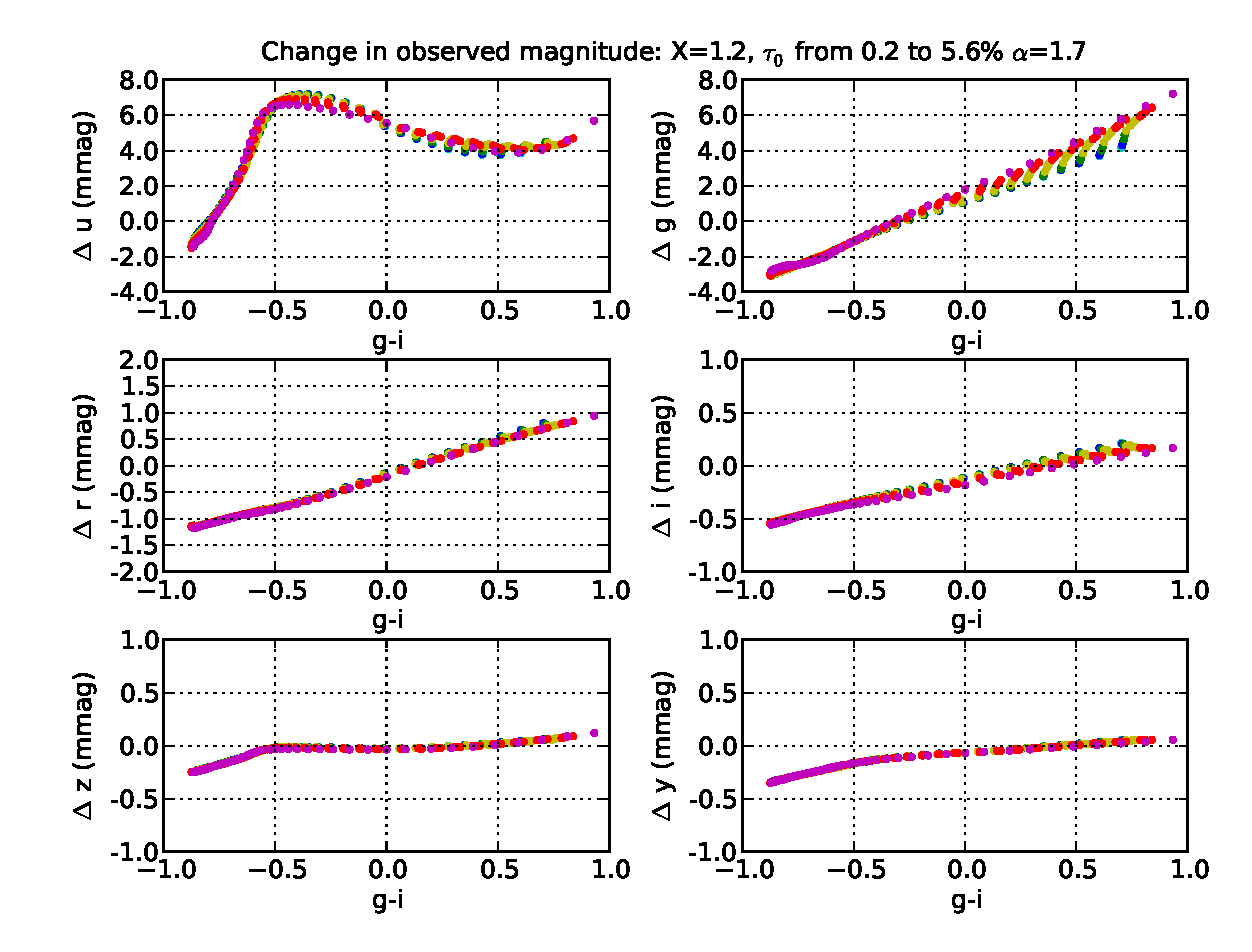
\includegraphics[width=3.2in]{delta_mags_t0full}}
\subfloat[]{\label{b}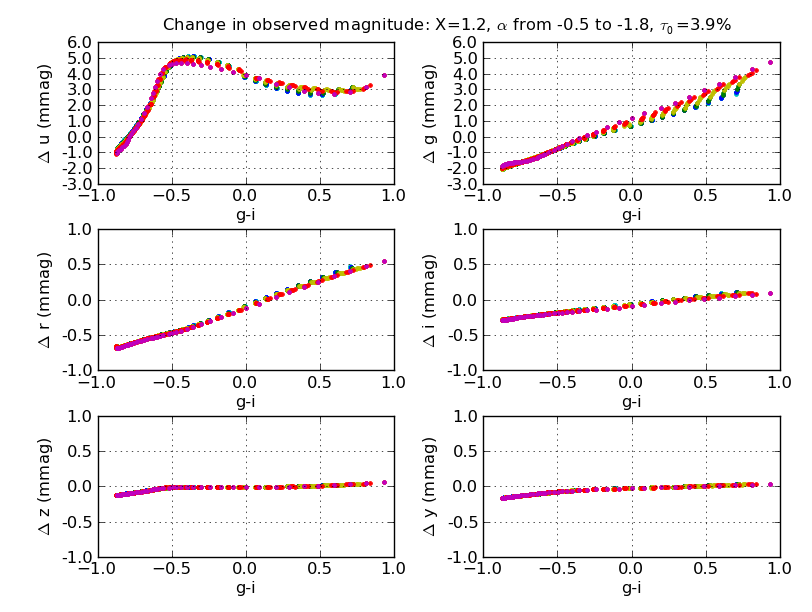
\includegraphics[width=3.2in]{delta_mags_alphafull}} \\
\subfloat[]{\label{c}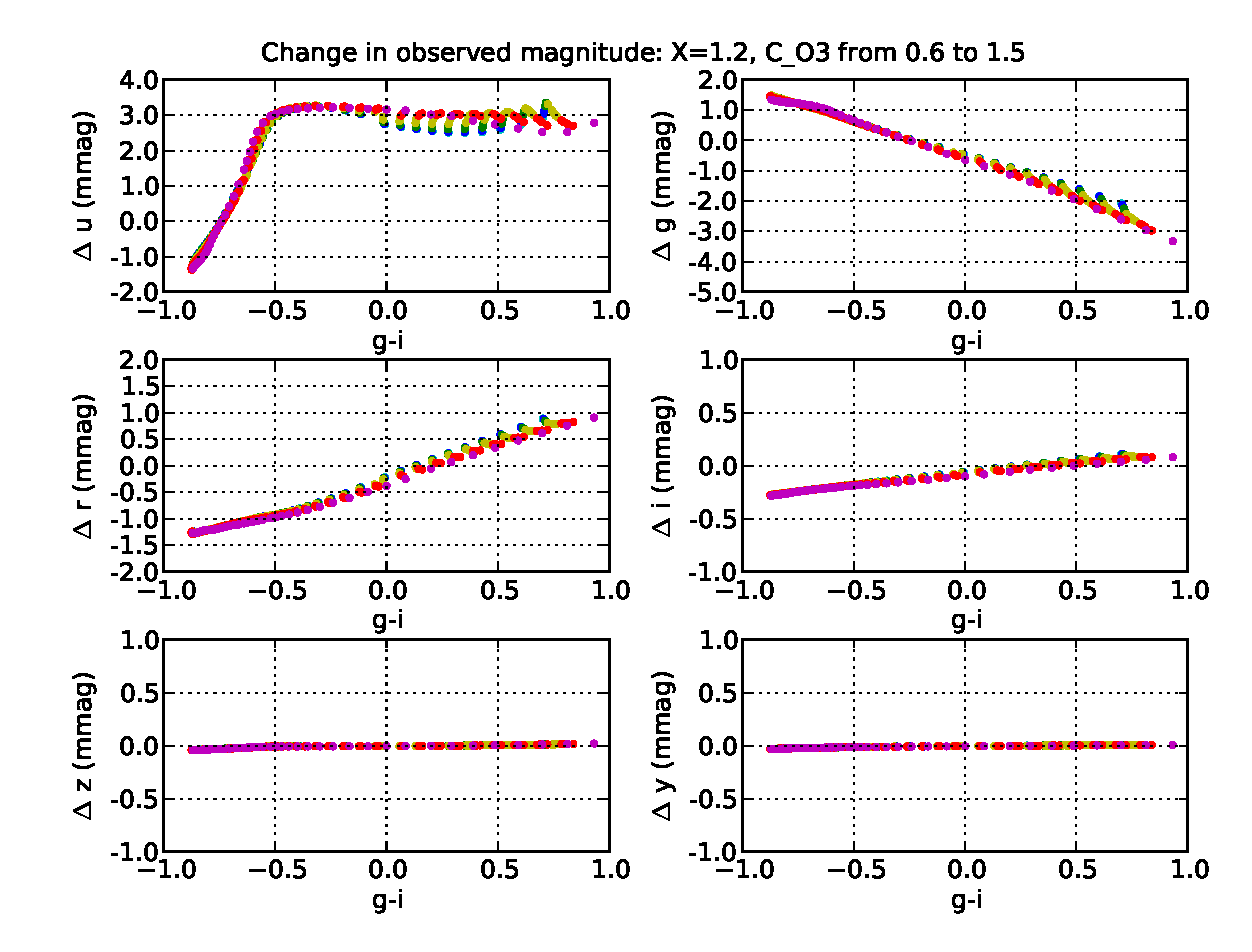
\includegraphics[width=3.2in]{delta_mags_O3full}}
\subfloat[]{\label{d}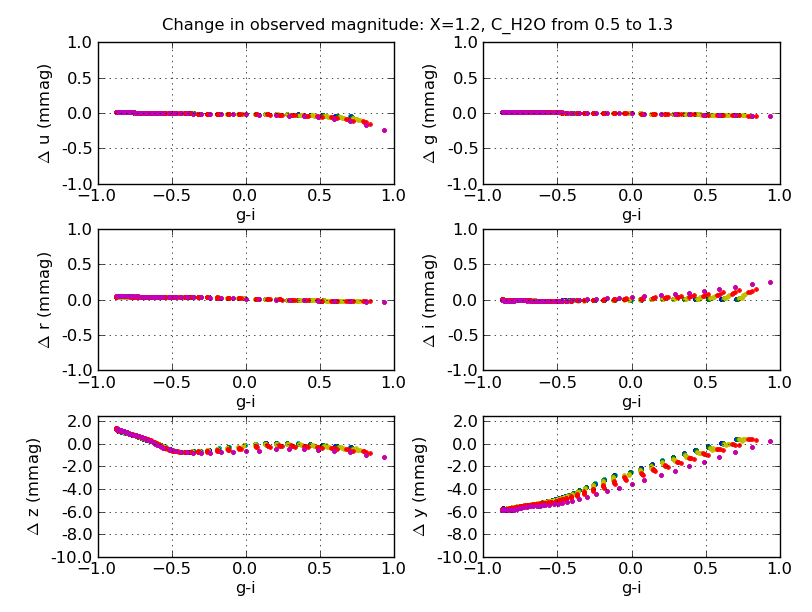
\includegraphics[width=3.2in]{delta_mags_H2Ofull}} 
\caption{{\small
{\bf $\Delta m_b^{obs}$ due to variations of each
individual absorption component.} Each atmospheric transmission curve
(at X=1.2) was combined with the set of main sequence Kurucz curves to
determine the resulting changes in observed magnitudes, as in
Figure~\ref{fig:dmag_filtershift}. \ref{a} and \ref{b} show the
effects of varying aerosol absorption in $\tau_0$ and $\alpha$
respectively, \ref{c} shows the effect of varying \ozone absorption. These
effects are concentrated in $u$ and $g$ bands, with a negligible effect
in $izy$. \ref{d} shows the effect of varying the \water absorption,
which is strongest in $y$, with some effect in $z$ and no effect in
$ugri$.
}}
\label{fig:dmag_atm_comps}
\end{figure}

\begin{figure}
\centering
\subfloat[]{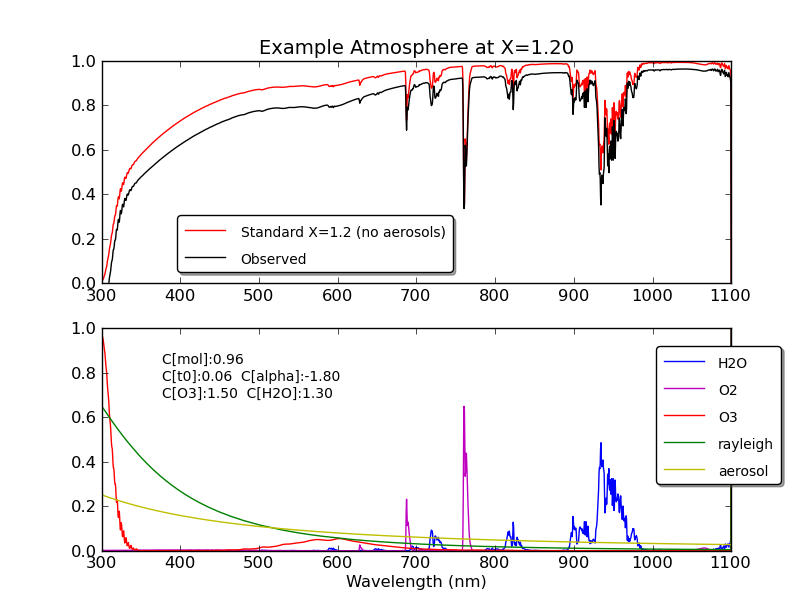
\includegraphics[width=5in]{atmo_max}} \\
\subfloat[]{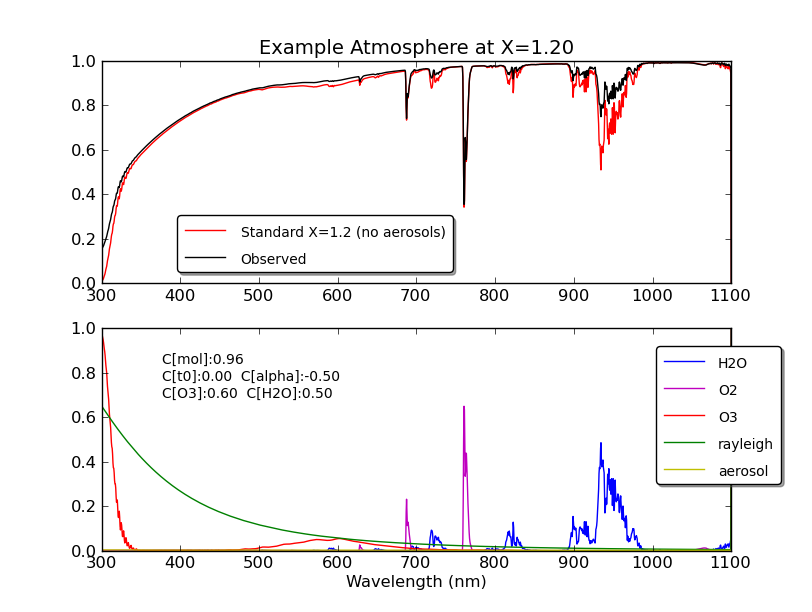
\includegraphics[width=5in]{atmo_min}}
\caption{{\small  {\bf `Extreme' atmospheres generated from MODTRAN profiles and extremes 
of atmospheric coefficients.} Using the extremes of $C_{\water}$, $C_{\ozone}$,
and $\tau_0$ and $\alpha$ from \citet{Burke2010b}, two test atmospheres
with $X=1.2$ were created using Equation~\ref{eqn:atmo_fit}. }}
\label{fig:atm_changes}
\end{figure}

\begin{figure}
\centering
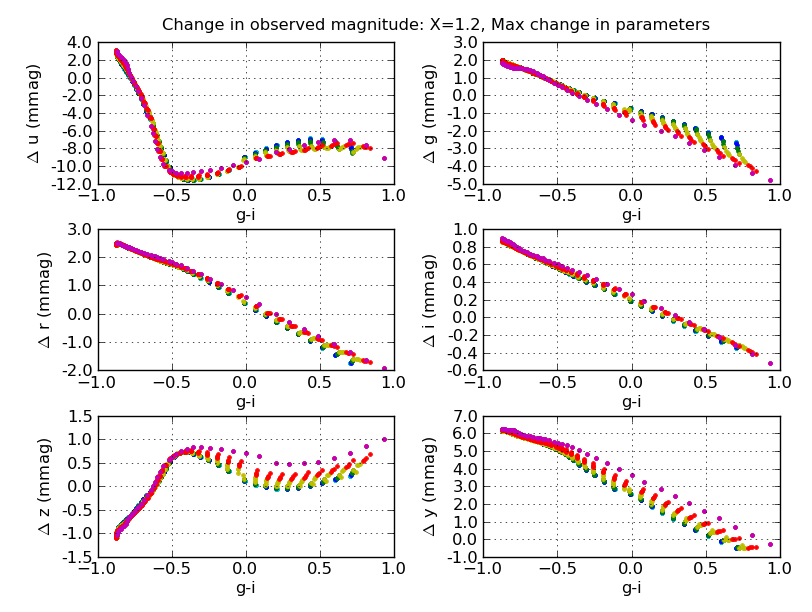
\includegraphics[width=6in]{delta_mags_max}
\caption{{\small
{\bf$\Delta m_b^{obs}$ due to `extreme' variations of 
atmospheric transmission.} Two atmospheric transmission curves were 
created using Equation~\ref{eqn:atmo_fit} and the widest variations of
atmospheric extinction coefficients from \citet{Burke2010b}. The wavelength
profile of these atmospheres is shown in Figure~\ref{fig:atm_changes}. 
These atmospheric transmission curves were combined with the baseline LSST 
hardware transmission curves, and used to generate magnitudes for 850 Kurucz
models with temperatures between 5000~K and 35000~K and metallicities between
-5.0 and 1.0 (solar). The resulting differences in natural magnitudes between 
the two extremes of the atmospheric transmission in each filter are shown above. 
}}
\label{fig:dmag_atm_max}
\end{figure}

\begin{figure}
\centering
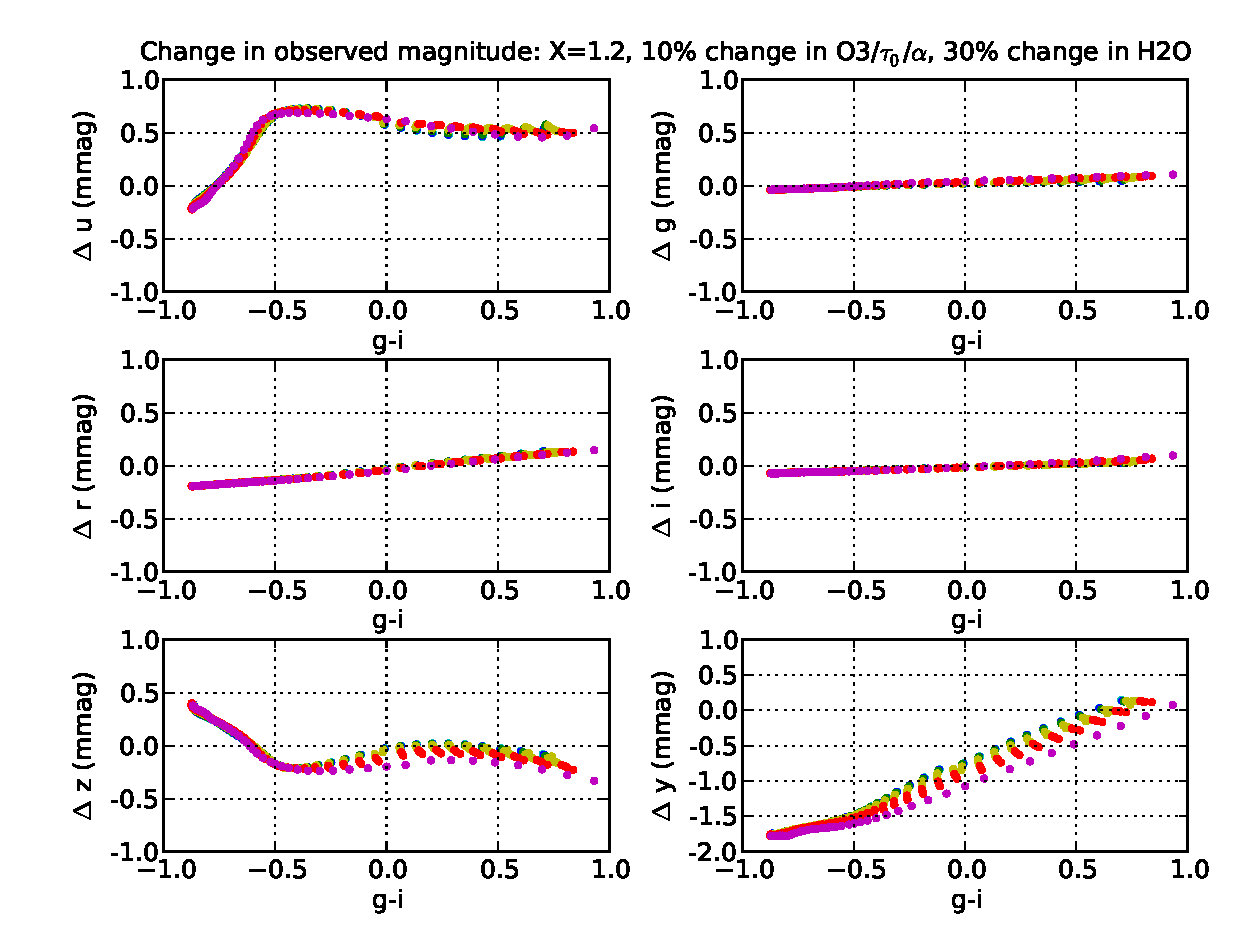
\includegraphics[width=6in]{delta_mags_10}
\caption{{\small
{\bf $\Delta m_b^{obs}$ due to 10\% variations of 
atmospheric transmission in \ozone and aerosol, with 30\% variation of \water.} 
This is similar to Figure~\ref{fig:dmag_atm_max}, except $C_{\ozone}$,
$\tau_0$ and $\alpha$ were only varied by 10\% of the total range of
values measured in \citet{Burke2010b}, and $C_{\water}$ was varied by 30\%
of the total range. }}
\label{fig:dmag_atm_10}
\end{figure}

Changes in airmass have a larger effect on observed natural magnitudes
(Figure~\ref{fig:dmag_airmass}) than the variation in atmospheric
extinction coefficients. However, these are included in the atmospheric extinction
templates generated by MODTRAN and can be accurately corrected.
Within the LSST $3.5^\circ$ diameter field of view, the difference in
airmass from top to bottom of the field can be considerable, and must
be included in the model. 

\begin{figure}
\centering
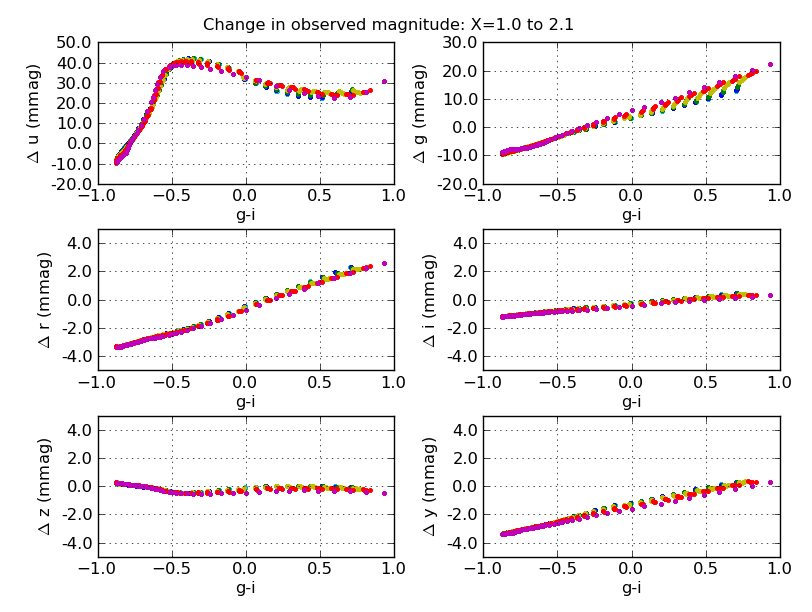
\includegraphics[width=6in]{delta_mags_airmass_big}
\caption{{\small
{\bf $\Delta m_b^{obs}$ due to changes in airmass from $X=1.0$ 
to $X=2.1$, for a typical atmospheric transmission response curve.}
}}
\label{fig:dmag_airmass}
\end{figure}


\subsubsection{Errors in the shape of the hardware and atmospheric response}
\label{sec:apply_deltak}

Correcting observed counts for the difference between the measured
shape of the hardware and atmospheric response curves and the standard
normalized bandpass, $phi_b^{std}(\lambda)$, requires knowledge of the
SED of each star. However, with this knowledge, it is possible to
create lookup tables of $\Delta m_b^{meas}(x,y,alt,az,SED,t)$ (as
in Equation~\ref{eqn:magsFromCounts}) for various locations in the focal
plane in each exposure. A rough example is given in
Table~\ref{tab:delta_mags}.

Assuming that the errors in the combined shape of the hardware and atmospheric
response curves add in quadrature, with the limits described above (2~mmag error
in $grizy$,  5~mmag error in $u$ due to the hardware response curve; 
1~mmag in $ugriz$, 2~mmag error in $y$ due to the atmospheric response curve), 
the final error in observed magnitude due to both of these effects would be $<3$~mmag
in $grizy$ and 5~mmag in $u$. There is an additional potential source of error in these
$\Delta m_b^{meas}$ corrections -- the understanding of the true SED of the 
source. 


\subsection{Normalization of the Atmospheric Transmission}
\label{sec:atmo_norm}

After applying each of the previous corrections, the raw counts have been
corrected to a `standard' bandpass for each filter,
$\phi_b^{std}(\lambda)$, using both the narrow band flats and the
atmospheric model derived from the auxiliary telescope
observations. Small scale ($<$ several times the PSF) gray-scale
zeropoint variations have also been removed by the synthetic
flat. However, there still remain variations in the normalization of the
system response that result from gray-scale extinction due to
clouds. The self-calibration procedure is necessary to correct for
these zeropoint offsets.

The self-calibration procedure selects bright, isolated main sequence
and white dwarf stars (or any star with well-known colors and a
well-known SED, to reduce errors in the applied
$\delta k$ values) from the sample of all observed stars after they are
corrected to the standard bandpass (`standardized'). Only non-variable stars will be
selected for self-calibration, based on approximately calibrated data
(say, a few percent) which will suffice in this context. It then uses
the many repeat observations $j$ of each star $i$ in a particular filter to minimize
\begin{equation}
\label{eqn:selfcalmin}
\chi^2 = \Sigma_{ij} \left(  { m_{b,ij}^{std} - m_{b,ij}^{model} \over
    \sigma_{b,ij}^{std} } \right)^2
\end{equation}
where the $m_{model}$ includes any remaining photometric corrections
that must be applied. In our current calibration plan, this would be only the
gray extinction from clouds, applied by requiring the photometric
zeropoint offset over a small patch of sky in a given observation, $\delta z_j$, be constant:
\begin{equation}
\label{eqn:zp}
m^{model}_{b,ij} = m^{best}_{b,i} - \delta z_{b,j},
\end{equation}
where the patch size is approximately one CCD in size. A more
complicated model, {\it e.g.} a $\delta z_{b}$ with structure, could
be used if found desireable. Simulations of the Milky Way based on a
model by Mario Juric (JuricREF) indicate that there will be
approximately 50--100 
suitable calibration stars per patch over the entire sky. 

Minimizing Equation~\ref{eqn:selfcalmin} requires solving for
approximately, $10^8$ $m_{b,i}^{best}$ and $10^8$ $\delta z_j$. Of
course, not all stars will be observed on all calibration patches, so
there will be only about 10$^{10}$ non-zero values of
$(m_b^{std})_{ij}$ (per band). Preliminary work using a conjugate
gradient method to compute $m_{b}^{best}$ and $\delta z_j$ for
approximately $10^6$ stars and $10^6$ patches was very successful; the
same method could be relatively easily parallelized for the full data
set. 

With the known values of $(\delta z)_j$, all measurements from that
patch can be re-calibrated, then analyzed for systematics in
$[(m_b^{std})_{ij} - (m_b^{best})_{i}]$ and $[(m_b^{obs})_{ij} -
(m_b^{best})_{i}]$ residuals (e.g., as a function of observation time,
position on the focal plane, airmass, seeing, stellar color,
brightness, seeing, etc.). The self-calibration step can be repeated
if necessary, with corrections for systematics incorporated in the
next-iteration values for $(m_b^{std})_{ij}$ or added directly into
the model magnitudes used for the self-calibration solution. Thus this
step provides a potential avenue for improvement in errors introduced
at earlier stages (such as a mis-measurement of the atmospheric
throughput or flat-field). 

The self-calibration step can be successful only if patches
overlap on the sky so that the same star is observed on 
multiple patches. It is good to note that $(m_b^{best})_{i}$ and 
$(\delta z)_j$ are constrained only up to an arbitrary 
additive constant. For convenience, this constant can be set so that
stars have roughly correct AB magnitudes, however the goal after
self-calibration is only to have a rigid, self-consistent magnitude
system, equivalent to the natural magnitudes.

More details of the self-calibration procedure can be found in
Docushare Document-8619 and Jones 2010 (SPIE paper). 


LJ - there is more to go here. Perhaps figure with milky way density 
in all bandpasses.  Definitely more info from more recent sims
that follow error distribution up to this point. Also describe some 
limits to selfcal. 

\section{Fixing LSST to an external scale}
\label{sec:calib_external}

The next two subsections describe how the internally calibrated
natural magnitudes, independently calibrated in each filter bandpass, are fixed
to an external scale such that the flux in a single band can be compared to the
flux in another filter band (SRD requirement \ref{color_req}) and that
the flux in a particular filter band can be compared to an absolute
external system (SRD requirement \ref{abs_req}). This is equivalent to
determining $\Delta_{br}$ and $\Delta_r$ from Eqn~\ref{eqn:extmags}. 

\subsection{Band to band (color)}

The band to band calibration for each filter $b$ (the $\Delta_{br}$
values) will be determined by measuring the flux from one or more
celestial objects whose physics and chemistry are believed to be well
understood. In principle, a single object with known colors would be
sufficient, however many objects across the LSST footprint
will be used to evaluate possible systematic effects in the internal
calibration process. 

Hot hydrogen (DA) and helium (DB) white dwarf stars have simple
atmospheres that are reasonably well understood (model colors are
currently reliable to about 0.01 magnitudes). It is estimated that
there will be $\approx$ 100/10 DA/DB WD stars with $r<24$ in each LSST
image at the South Galactic Pole. Catalogs of WD stars visible from
Cerro Pachon have been constructed (Bergeron 1992, Eisenstein
2006), and a `white dwarf calibration system' has been developed
(Holberg \& Bergeron 2006). The locus of main sequence stars in
color-color space is also reasonably well understood and has been used
to calibrate photometry with success in previous surveys (MacDonald
2004, Ivezic 2007). The use of the main sequence stellar locus in addition to
WD stars will provide a valuable check on systematic effects that may
arise from using (primarily) white dwarfs in the determination of
$\phi^{atm}(\lambda,alt,az,t)$. 

The values for $\Delta_{br}$ will be determined by generating model
$m_b^{nat}$ values for each band-band calibration object, then
minimizing 
\begin{equation}
\chi^2 = \Sigma_{i} \left( { (m_{b,i}^{nat} - m_{r,i}^{nat})^{meas} - (m_{b,i}^{nat}
    - m_{r,i}^{nat})^{model} \over  \sigma_{b-r,i}}\right) ^2. 
\end{equation}
This comparison can
be done using subsets of objects from low galactic extinction regions,
and then bootstrapping to the entire sky to check for systematic
effects, perhaps by using the main sequence stellar locus as an
additional method to determine the amount of galactic extinction. 

LJ - there is more to come here, based on notes from Zeljko. Include 
stellar locus / quasar locus / white dwarf locus and how this 
can help constrain band-to-band color variations (particularly with
different sensitivities to dust)

\subsection{Single bandpass to external flux system (absolute scale)}

After determining the band to band calibration, there is a single
number required to calibrate the entire system to an absolute flux
scale: $\Delta_r$.  This can again be determined using a single
object with a well-known flux and spectral energy distribution,
however multiple external calibrators provide a valuable check on
systematic effects. 

Several WDs in the Northern hemisphere have been very precisely
calibrated with HST STIS measurements (Bohlin \& Gilliland 2004) and
it should be possible to obtain similar HST measurements of one or
more targets for use in the Southern hemisphere. Identification of
these targets has not yet been done. 



\bibliographystyle{apj}
\bibliography{calib_plan}


\appendix

\newpage
\section{Filter Set}

\begin{figure}[h!]
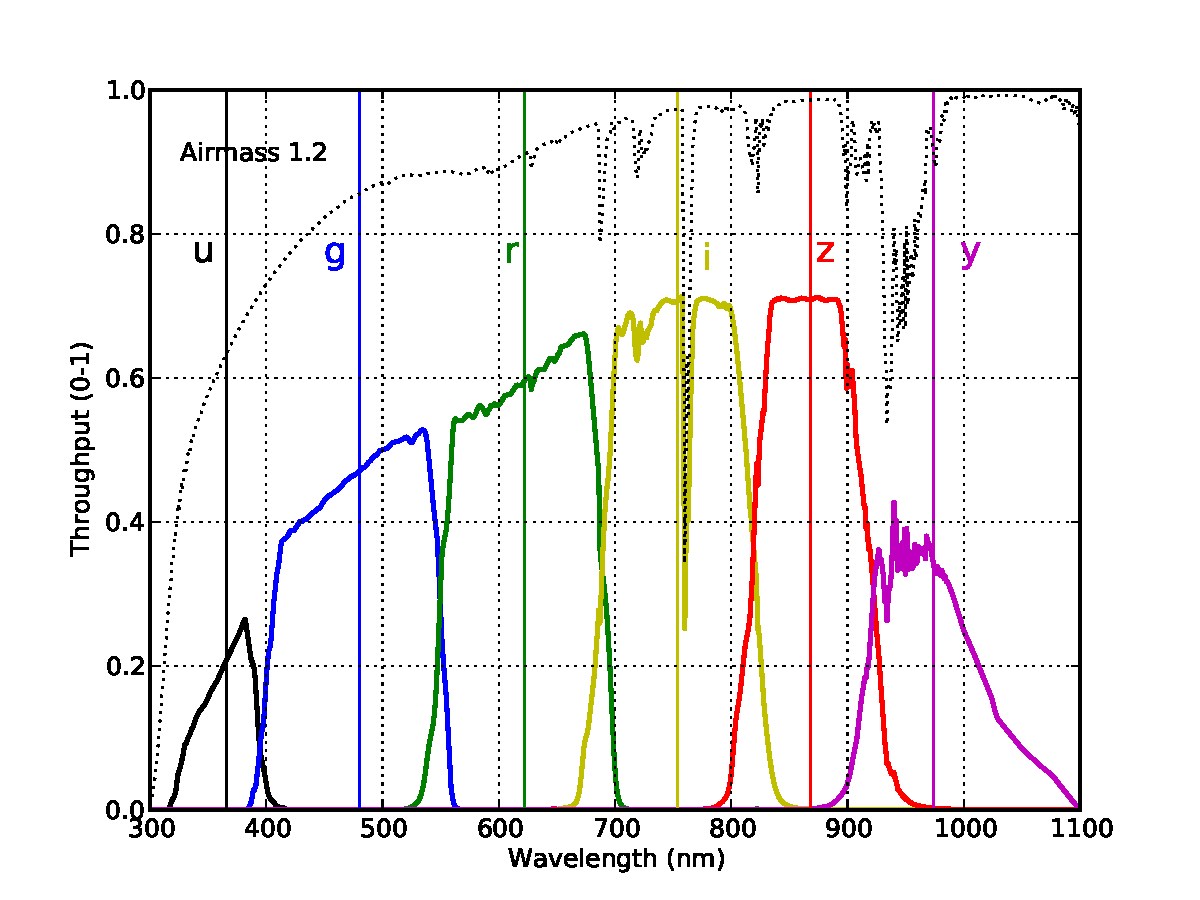
\includegraphics[width=5in]{filters}
\end{figure}


\section{Improvements in photometric accuracy}
\label{sec:photo_better}

LSST will record series of $m_b^{nat}$ measurements for each
astronomical object in each visit, resulting in approximately
$s\times10^{13}$ measurements. These $m_b^{nat}$ measurements are
generated directly from the counts recorded in each image, as well as
a normalization offset, which compensates for flat field changes, the
illumination correction, and gray (cloud) atmospheric extinction
effects.  However, these $m_b^{nat}$ measurements will vary as the
shape of the bandpass changes, whether as a function of position in
the focal plane or as a function of changes in atmospheric absorption
components. Correcting for these effects requires assuming a
particular SED for each source, and produces $m_b^{std}$ values after
applying $\Delta m_b^{meas}$ offsets (see the overview of calibration
in section~\ref{sec:counts2photons} for a review). 

In order to permit scientists to generate higher precision photometry
for objects using arbitrary SEDs, the value of
$\phi_b^{meas}(\lambda,alt,az,x,y,t)$ as well as the normalization
zeropoint offsets must be available. With these additional pieces of
information, scientists can generate more precise $\Delta m_b^{meas}$
corrections, using their own chosen object SED to generate
$m_b^{std}$.

For many objects, LSST will assume a flat SED when generating
$m_b^{nat}$ values, implying that no $\Delta m_b^{meas}$
correction was applied. Sections~\ref{sec:hardware_phi} and
~\ref{sec:atmo_phi} outline the typical magnitudes of these corrections;
for some main sequence stars these corrections can easily be on the
order of 20 mmag for $gri$, or even 100 mmag in $u$ band. For more
extreme SEDS, these corrections may be even
larger. Figure~\ref{fig:dmag_allseds} illustrates the likely magnitude of
these corrections for a variety of SEDs. In each plot, the main
sequence stars are shown as in the figures in the main paper (small
dots, color-coded by metallicity), although given the increased scale
here they only appear as a purple series of circles. M dwarfs are now
included, generally mimicking the behavior of the main sequence stars but
further into the red. More unusual SEDs are also
included; a quasar SED, based on a composite of many empirical quasars
from SDSS from \citet{VandenBerk2001} that has been extended to the
full LSST wavelength range through the addition of power law flux
above and below the original range ($f_\nu \propto 1/\lambda^{0.5}$
for $\lambda<89$nm \& $f_\nu \propto 1/\lambda^{1.5}$ for
$\lambda>800$nm), and redshifted from $z=0$ to $z=3$; also a sample of
SN Ia from templates generated by Peter Nugent \citep{Nugent2002}, redshifted
from $z=0$ to $z=1$.  

The figure shows the $\Delta m_b^{obs}$ values that would be expected
under a maximum change of atmospheric parameters and under a likely
bandpass shift. This also shows how much the reported $m_b^{nat}$
values could vary for each object. If LSST was to just calculate an
offset between $m_b^{nat}$ and $m_b^{std}$ based on an object's color
(and assuming that the object had an SED similar to a main sequence
star), the resulting $m_b^{std}$ values would be incorrect by the
value of the offset between the true $\Delta m_b^{obs}$ for the SED
and the main sequence $\Delta m_b^{obs}$ values at each color; this
could easily be more than 20mmag.  This is why applying $\Delta
m_b^{meas}$ values appropriate for each SED is required to generate
$m_b^{std}$ magnitudes precise to better than 1\%, and why LSST Data
Management must record $\phi_b^{meas}(\lambda,x,y,t)$ for each
observation. 

\begin{figure}
\centering
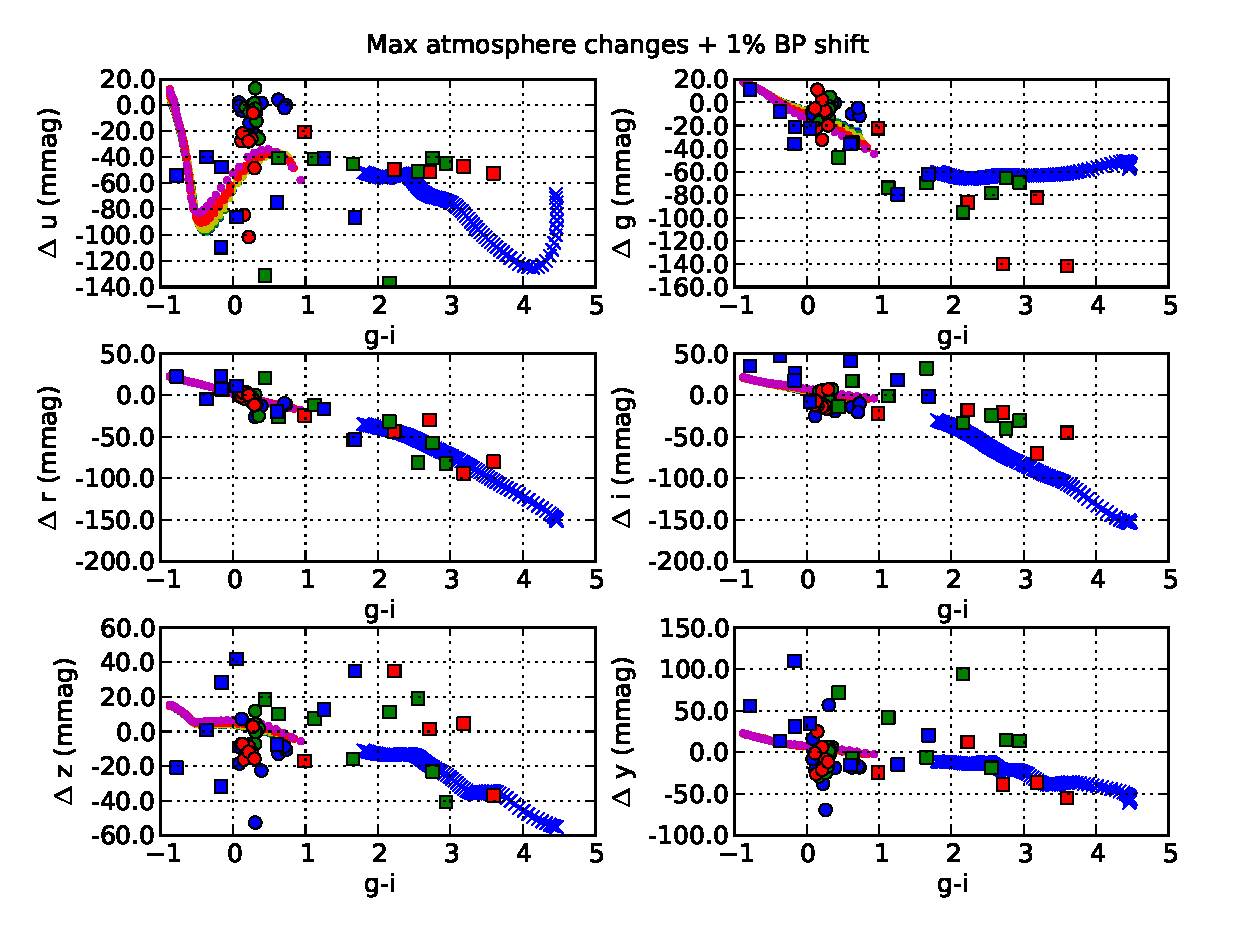
\includegraphics[width=6in]{dmag_all_max+shift}
\caption{{\small
{\bf $\Delta m_b^{obs}$ due to changes in a hardware bandpass shift
  and a maximum change in atmospheric absorption components.}  This
plot is similar in nature to a combination of
Figure~\ref{fig:dmag_filtershift} and \ref{fig:dmag_atm_max}, but has
been extended to include a wider variety of object SEDs. Main sequence
stars are shown as the sequence of purple dots, and Mdwarfs are
shown as the sequence of blue 'x's. The large round circles represent
a quasar SED at various redshifts, color-coded with redshift as
follows: $0<z<1$ is blue, $1<z<2$ is green, and $2<z<3$ is red. The
large filled squares show the change in natural magnitudes for SNIa
templates at times of 0, 20, and 40 days from peak; $0<z<0.36$ are
blue squares, $0.36<z<0.72$ are green squares, and $0.72<z<1$ SNIa are
red squares. 
}}
\label{fig:dmag_allseds}
\end{figure}


%\section{Comparison of standard calibration and SDSS ubercal (as
% approximation for this method)}


%\section{Thermal IR Camera}
%possibility to generate measurement of shape of cloud structure over
%field of view (could function as prior for self-calibration)

%if cloud structure found to vary on scales smaller than length between
%calibration stars (or minimum scale possible to correct with
%self-calib), then thermal IR camera would enable generation of
%these corrections

%may provide useful SDQA data (especially for alerts/nightly data
%stream)


\section{Glossary}
\label{sec:glossary}

\begin{itemize}

\item{{\bf Level 1 Data Product.} A data product, such as a measurement
  of an astronomical object's position or flux in a single image, that
is computed on a nightly basis. Level 1 data products primarily
consist of alerts on transient, variable and moving objects. The
photometric calibration process outlined in this paper does not apply
to Level 1 data products. Level 1 data products will be calibrated
using all applicable prior knowledge (including secondary standard
catalogs generated from previous Data Release calibration of all
LSST-observed stars in the field). }

\item{{\bf Level 2 Data Product.} A data product, such a measurement
    of an astronomical object's position or flux in either a single
    image or a series of images, that is computed on the Data Release
    schedule, on a six-month or yearly schedule. Level 2 data products
    leverage all previous observations of the same object, as well as
    all knowledge of the LSST system accumulated to that point. The
    photometric calibration process outlined in this paper is used to
    generate Level 2 data products. }

\item{{\bf Normalized system response, $\phi_b(\lambda)$.} The
    normalized system response describes the shape of the bandpass
    transmission curve, separating this from the normalization of the
    throughput curve which can be determined separately.
    $phi_b(\lambda)$ is described by Equation~\ref{eqn:PhiDef}. The
    integral of $phi_b(\lambda)$ is always 1. }

\item{{\bf Illumination Correction.} }

\item{{\bf Natural magnitude.}} 

\item{{\bf Standard magnitude.}}

\end{itemize}


\end{document}
